% !TEX program = pdflatex
% When Scalar Diffraction Theory Fails: RCWA-Calibrated Physics-Anchored
% Inverse Design of Polymer AR Waveguide Couplers
%
% Formatted to standard IEEE conventions (two-column, Times, numbered
% bracketed citations, Roman-numeral ALL-CAPS section heads, Abstract +
% Index Terms block, standard back-matter) using the standard article
% class with titlesec-based section heads in place of IEEEtran.cls.
% Swapping in IEEEtran.cls is a one-line \documentclass change if a venue
% requires the literal template.
%
% Revision 3 (2026-07-17). Every quantitative claim in this manuscript was
% independently derived by the author from the project's source files and
% checkpoints; the verification scripts and their output are archived
% alongside this file.

\documentclass[10pt,twocolumn]{article}
\usepackage[utf8]{inputenc}
\usepackage[T1]{fontenc}
\usepackage[margin=0.75in,columnsep=0.25in]{geometry}
\usepackage{times}
\usepackage{amsmath,amssymb}
\usepackage{graphicx}
\usepackage{booktabs}
\usepackage{array}
\usepackage{titlesec}
\usepackage{enumitem}
\usepackage[hidelinks]{hyperref}
\usepackage{cite}
\usepackage{textcomp}
\usepackage{caption}

\captionsetup{font=footnotesize,labelfont=bf}
\setlength{\parindent}{1em}
\setlength{\parskip}{0pt}

% ---- IEEE-style section headings -------------------------------------
\titleformat{\section}{\centering\normalfont\small\bfseries}{\Roman{section}.}{0.5em}{\MakeUppercase}
\titleformat{\subsection}{\normalfont\small\bfseries}{\Alph{subsection}.}{0.5em}{}
\titleformat{\subsubsection}{\normalfont\itshape\small}{\arabic{subsubsection})}{0.5em}{}
\titlespacing*{\section}{0pt}{2.0ex plus 1ex minus .2ex}{1.2ex plus .2ex}
\titlespacing*{\subsection}{0pt}{1.5ex plus 1ex minus .2ex}{1ex plus .2ex}

\renewcommand{\refname}{References}

\begin{document}

\twocolumn[
\begin{@twocolumnfalse}
\begin{center}
{\LARGE\bfseries When Scalar Diffraction Theory Fails: RCWA-Calibrated,\\[2pt]
Physics-Anchored Inverse Design of Polymer AR Waveguide Couplers\\[10pt]}
{\large Connor Wang\\[2pt]}
{\normalsize\itshape Independent Researcher\\[4pt]}
{\footnotesize Handling Editor: Andrew Ho\\[8pt]}
\end{center}

\begin{center}
\begin{minipage}{0.92\textwidth}
\small
\textbf{Abstract}: In a full-color, single-layer, low-index polymer
waveguide, the total-internal-reflection guiding condition forces the
in-coupling grating's period below every visible design wavelength, which
is exactly the sub-wavelength regime in which scalar diffraction theory is
known to break down. We show that this is not a rounding error: at the
period a scalar-theory-guided search selects for a poly(methyl
methacrylate) (PMMA) combiner, rigorous coupled-wave analysis (RCWA)
reports first-order coupling efficiency $5.1\times$ lower at 532~nm and
$15.7\times$ lower at 635~nm than the scalar model claims, and correcting
the coupling term moves the true efficiency optimum off the scalar model's
400~nm depth bound to an interior optimum near 200~nm. We build a
differentiable analytic system engine (TIR guiding, polarization-resolved
Fresnel and roughness losses, a five-term MTF cascade) whose grating-coupling
term is replaced with a multilinear interpolant over 90,090 rigorous RCWA
solutions spanning refractive index, period, depth, and duty cycle (global
mean interpolation error $5.6\times10^{-4}$ against 48 off-grid solves), and
use it as the frozen decoder in a tandem neural inverse-design network that
maps a target system specification directly to a waveguide design, alongside
a forward surrogate and a neural-adjoint search. On 20{,}000 freshly sampled
held-out specifications the tandem network resolves the field's standard
one-to-many inversion failure: median per-metric relative error of $1.3\%$
(MTF) to $9.9\%$ (transmission), against $11.9\%$ to $49.1\%$ for a
direct design-regression baseline trained without the physics decoder in
the loop. A neural-adjoint search over the trained surrogate and an
independent gradient search directly on the exact physics converge, from
hundreds of random restarts each, on the same design (grating depth
$\approx 200$~nm, period $448$~nm, duty cycle $\approx 0.42$-$0.44$), whose
coupling efficiency we re-verify with a dedicated rigorous electromagnetic
solve at $41\%$ higher (unpolarized) than the true, rigorously
re-evaluated efficiency of the design a scalar-theory-driven search would
have shipped instead; because the record design is, in its own right, an
effectively TE-only coupler ($96.9\%$ of coupled power, Section~VI-F), the
more representative comparison is TE-to-TE, where the gain is $3.4\times$
rather than $41\%$, and pairing the design with an already-polarized
projector source (LED or LCoS) recovers a further $1.9\times$ transmission
gain at no geometry cost. Absolute double-coupler transmission at this
design is $1.25\%$, consistent with the single-digit system efficiencies
reported for conventional diffractive AR combiners in the literature; a
naive comparison against a scalar-theory transmission estimate at the old,
scalar-optimal geometry gives a $8.9\times$ apparent drop, a number we
report and scope carefully (Section~VI-D) rather than lead with, since it
compares a wrong estimate at one geometry against a correct measurement at
a different one and is not, by itself, evidence of a regression. The reported design is a
spin-coated PMMA surface specifically ($\sigma\approx0.7$-$1.1$~nm, following
measured polymer-waveguide roughness values in the literature); evaluating
the same geometry at the reported roughness of an uncoated polymer surface
lowers transmission by roughly a third, which we quantify explicitly rather
than describe the design as coating-free. We also find that the record
design's chromatic-blur term sits within the top few percent of what its
governing metric can achieve under random guided-angle phase, and that this
term oscillates rapidly enough in spatial frequency that the design's
evaluation frequency lands on a constructive fringe rather than a
representative value, a concrete instance of a differentiable image-quality
metric being tunable rather than merely satisfied. The framework and its
validation protocol, physics-probe checkpoint invalidation, a memorization
audit, and independent verification of every headline design in an
electromagnetic solver, are offered as a template for physics-honest,
system-level inverse design of consumer-grade polymer waveguides, together
with an explicit account of where that honesty still falls short.

\smallskip
\textbf{Index Terms}: augmented reality, diffractive waveguide,
inverse design, tandem neural network, rigorous coupled-wave analysis,
surface-relief grating, physics-informed machine learning.
\end{minipage}
\end{center}
\bigskip
\end{@twocolumnfalse}
]

\section{Introduction}

A diffractive waveguide combiner routes a projector image into a thin,
mostly-transparent slab of glass or plastic using a pair of surface-relief
gratings: one couples light in and traps it by total internal reflection,
the other lets it back out toward the eye. It is the optical architecture
behind most of the AR glasses shipping today, because it is thin, can be
mass-produced, and does not obstruct the wearer's view of the real world
\cite{kress2021}. The trouble is that its image quality, meaning
sharpness, brightness, and the amount of rainbow fringing at the edge of
the field of view, is a tangled function of eight-odd
material and geometric parameters: refractive index, absorption, surface
roughness and its correlation length, slab thickness, and the grating's
period, depth, and duty cycle. Changing any one of them to fix one metric
typically moves the other three. Waveguide designers have historically
handled this by hand-tuned parameter sweeps or, more recently, by
gradient-based optimization of a physics or electromagnetic model directly.

Over the last two years a handful of groups have instead trained neural
networks to invert this relationship: given a target optical performance,
output the waveguide geometry that achieves it, in a single forward pass
rather than an iterative search. The dominant recipe, borrowed from the
broader nanophotonic inverse-design literature \cite{liu2018,peurifoy2018,
ma2021}, is the \emph{tandem network}: train a forward surrogate to emulate
an expensive simulator, freeze it, and train a second network to output a
design by backpropagating a loss computed in performance space through the
frozen surrogate. This sidesteps the central difficulty of design inversion:
many different geometries can produce nearly the same
optical output, so regressing directly from performance to geometry trains
against a target that is not really a function.

Recent waveguide-specific applications of this recipe invert a single
component-level quantity: the RGB coupling-efficiency spectrum of a slanted
grating, learned from rigorous coupled-wave analysis (RCWA) simulations
\cite{luo2024}; the exit-pupil brightness uniformity of a head-up-display
combiner, with a reported $40{,}000\times$ speedup over the RCWA sweep it
replaces \cite{dai2025}; or the reflection spectrum of a hybrid grating
stack, using a tandem network alongside a conditional variational
autoencoder to also recover design diversity \cite{dehghani2025}. In every case
the forward model inside the tandem is itself a learned surrogate for RCWA
or a ray tracer, so the training signal the inverse network chases already
carries the surrogate's approximation error, and none of them close the
loop from a single component metric up to the perceptual, system-level
quantities (sharpness, color fringing, brightness at the edge
of the field of view) that actually describe what a wearer
sees.

This work targets that gap along two axes at once. First, we invert a
\emph{multi-metric system-level specification} evaluated simultaneously
rather than a single component metric: MTF at 40~cyc/mm, total
double-coupler transmission, an internal guided-mode angle spread across
the RGB primaries (a quantity we relabel from an earlier, imprecise
``lateral chromatic spread'' following independent review, Section~III-B),
and transmission at the field edge. We are explicit, and more explicit than
in this manuscript's first draft, that the last of these four is closely
tied to total transmission by construction (Section~III-C) rather than
fully independent evidence, and that the guided-angle spread is not itself
a validated model of retinal color error; Section~III-A states precisely
what this specification vector does and does not capture. Second, we anchor
the tandem's decoder to an \emph{exact differentiable analytic physics
engine}, a PyTorch implementation of a closed-form system model (grating
equation, polarized Fresnel transmission, a roughness scattering loss in
the spirit of Tien \cite{tien1971} and Bennett and Porteus
\cite{bennett1961}, and a five-term MTF cascade including the exact
chromatic point-spread treatment of Thibos \cite{thibos1987}), validated
term by term against the literature closed forms and against rigorous
electromagnetics directly in this paper (Section~III), rather than a second
learned surrogate. That removes one whole source of approximation
error from the training signal: every gradient the inverse network sees is
physically interpretable, not an artifact of how well a second network
happened to fit its own training set.

A material choice this framework makes and does not revisit is PMMA
itself, and it is worth addressing directly rather than leaving implicit,
because the guided-window analysis in Section~III shows that PMMA's low
index is precisely what narrows the full-color field of view to a few
degrees (Section~III-A). Higher-index resins exist and are used
specifically to relax this constraint: Luo and Lee's slanted-grating design
\cite{luo2024} uses an episulfide resin with $n\approx1.70$-$1.72$ for this
reason. PMMA remains the substrate of interest here for the properties a
narrow-FOV, cost- and weight-constrained device trades on: it is
substantially cheaper and lighter than glass or high-index resin, is
compatible with roll-to-roll and injection-molding manufacturing rather
than precision optical polishing, and is far more impact-resistant, the
reasons plastic combiners have already shipped in commercial holographic
AR products \cite{yoshida2018}. This trade is not free of competition:
single-layer, full-color silicon-carbide waveguides ($n\approx2.6$) have
been demonstrated at sub-millimeter thickness and gram-scale mass with a
wide field of view and no rainbow artifact \cite{chen2025sic}, directly
undercutting a cost/weight argument for low index made in isolation. We
do not attempt a cost or manufacturability comparison in this paper, and
do not claim PMMA wins that comparison against SiC or other emerging
high-index platforms; we report PMMA's optical consequence, a narrow
full-color guided field of view, as a real, quantified constraint of the
material rather than a defect of the modeling, and leave the
cost-versus-field-of-view trade, now including SiC as a live alternative,
explicitly to the reader's application (Section~VII).

A differentiable analytic engine is not automatically an honest one,
though, and the second contribution of this work is finding and fixing the
place where ours was not. The engine's grating-coupling term originally
used the standard scalar binary-phase-grating formula from Fourier optics
\cite{goodman}. That formula is accurate for features much larger than the
wavelength of light; Pommet, Moharam, and Grann showed in 1994 that its
error exceeds five percent once the feature size drops below about
fourteen wavelengths \cite{pommet1994}. The guided-window constraint we
derive in Section~III, the geometric condition a grating
period must satisfy for the diffracted beam to actually stay trapped in
the slab, forces PMMA's period into a window of roughly
430\textendash449~nm for full-RGB operation: below the wavelength of every
color in the design. We are, in other words, optimizing a design deep
inside the regime scalar theory is known to get wrong, and the resulting
error is not a rounding issue: at the design our own scalar-theory-driven
search converged to, rigorous electromagnetic simulation shows the true
coupling efficiency is five to sixteen times lower than the scalar model
reported, and the true optimum sits at a different grating depth entirely.
Section~IV describes how we replaced the scalar term with a coupling
efficiency calibrated to 90,090 rigorous solutions and what changed once we
did.

Shipped and reported polymer diffractive waveguides exist
\cite{nilsen2025}, so we do not claim PMMA inverse design itself is new;
what we have not found elsewhere in this literature is a system-level
(rather than component-level) specification paired with a coupling term
calibrated against rigorous electromagnetic simulation rather than trained
on it, applied to PMMA's full-color guiding constraint specifically. We
verify every headline design independently in a
second, dedicated rigorous solve, and we run an explicit memorization audit
on the forward surrogate rather than reporting only a validation-set
$R^2$. Section~VIII is a candid accounting of what has \emph{not} yet been
done: an out-of-distribution generalization test, a
reverse-engineering case study against a published commercial-class
specification, and the remaining seeds of a planned five-seed statistical
protocol. We include it because a paper that calibrates against exact
electromagnetics ought to be equally exact about its own scope.

\section{Related Work}

Table~\ref{tab:related} summarizes the closest prior neural inverse-design
work for waveguide gratings and displays, alongside the broader tandem and
neural-adjoint methods this work builds on. The field's current
best-in-class result sits outside this table's scope: Gopakumar et al.\
pair inverse-designed metasurface waveguides with an AI-driven holographic
light engine for full-color, 3D, large-\'etendue augmented reality from a
glasses-like form factor \cite{gopakumar2024}, a system-level achievement
this paper's single in/out-coupler-pair, 2D-content model (Section~III-A)
does not attempt to approach; we cite it as context for how far the
field's frontier has moved, not as a directly comparable baseline. Ding,
Yang, Li et al.\ survey the broader waveguide-combiner landscape,
perspectives, and open challenges as of 2023 \cite{ding2023elight}.

Liu, Tan, Khoram, and Yu introduced the tandem architecture for
nanophotonic inverse design: rather than regress geometry directly from a
target spectrum, which fails when many geometries share a spectrum, train
an inverse network through a frozen, pretrained forward surrogate so the
loss is computed in a well-posed output space \cite{liu2018}. Peurifoy et
al.\ demonstrated the companion half of the recipe, training a forward
surrogate to replace an electromagnetic simulator for nanoparticle
scattering and using it for gradient-based inverse design directly
\cite{peurifoy2018}. Ren, Padilla, and Malof formalized and benchmarked the
\emph{neural-adjoint} variant used in Section~V-C of this work: freeze a
trained forward surrogate, treat the design parameters themselves as the
optimization variables, and run gradient ascent through the network's
weights from many random restarts \cite{ren2020}. Ma et al.\ survey this
surrogate/tandem/adjoint taxonomy across the broader photonic
inverse-design literature \cite{ma2021}.

Within waveguide combiners specifically, Luo and Lee train a tandem network,
an invertible, generative-flow-based network paired with a
fully connected regressor, to invert the RGB coupling
efficiency spectrum of a slanted grating from RCWA-simulated training data
\cite{luo2024}. Dai et al.\ train a neural network, refined with Bayesian
and particle-swarm optimization, to invert the exit-pupil brightness
uniformity of an AR head-up-display waveguide, reporting a $40{,}000\times$
speedup over the simulation sweep it replaces at better than 97\% accuracy
\cite{dai2025}. Dehghani et al.\ train a tandem network and a conditional
variational autoencoder side by side to invert the reflection spectrum of
a hybrid grating stack from noisy measurements, using the cVAE specifically
to recover the diversity of near-equivalent designs that a deterministic
tandem network collapses to a single point \cite{dehghani2025}. On the
achromatic-coupler side, Tian et al.\ demonstrate a full-color AR system
built around an inverse-designed achromatic metasurface coupler paired with
a high-index waveguide, solved with a full-wave (not tandem-network) method
\cite{tian2025}. Closer to a full system treatment, Lee, Lee, and Chung use
adjoint-based optimization, not a tandem network, to design triple-function
metasurface couplers that explicitly target chromatic dispersion, ghost
orders from parasitic diffraction, see-through scene distortion, and
eyebox uniformity together \cite{lee2025nanophotonics}: this is the most
complete system-level treatment we are aware of in this literature, and it
addresses several image-quality failure modes (ghosting, see-through
distortion, exit-pupil expansion) that the present specification vector
does not model at all (Section~III-A). It targets a general high-index
metasurface coupler rather than a low-cost polymer substrate and uses
direct adjoint optimization of the electromagnetic solver rather than a
trained tandem network for repeated, fast specification-to-design queries;
those are the two axes on which this paper's contribution is scoped, not a
claim to a broader system-level treatment than \cite{lee2025nanophotonics}
achieves.

Every one of the tandem/surrogate-based waveguide works above inverts a
single component-level quantity (a coupling spectrum, a pupil
uniformity map, a reflection spectrum) through a forward model
that is itself a learned surrogate for RCWA or a ray tracer. None combines
a multi-metric, system-level specification with a tandem network whose
decoder is exact physics rather than a second learned network, though
\cite{lee2025nanophotonics} reaches a comparable system-level scope by a
different (adjoint, non-tandem) route and covers more failure modes than
this paper does. Zhao et al.\
derive a reciprocity- and energy-conservation-based upper bound on
in-coupler efficiency that we use in Section~VII to contextualize our
absolute transmission numbers, rather than as a design method
\cite{zhao2024}. Kress and Chatterjee's review of waveguide combiner
architectures is the system-level framing this paper's specification
vector is drawn from \cite{kress2021}. Nilsen et al.\ report the PMMA
material parameters (index, roughness statistics) this work draws its
design bounds from \cite{nilsen2025}.

\begin{table*}[t]
\centering
\caption{Positioning against the closest prior neural inverse-design work for AR waveguide combiners.}
\label{tab:related}
\footnotesize
\begin{tabular}{p{2.9cm}p{2.7cm}p{2.7cm}p{7.0cm}}
\toprule
\textbf{Work} & \textbf{Inverts} & \textbf{Forward model} & \textbf{Positioning} \\
\midrule
Luo \& Lee, \emph{Opt.\ Express} 32, 12587 (2024) \cite{luo2024} & RGB coupling efficiency of a slanted grating & Learned (RCWA-trained) & Component-level only; carries surrogate approximation error \\
Dai et al., \emph{Appl.\ Opt.} 64, 3536 (2025) \cite{dai2025} & Exit-pupil brightness uniformity & Learned neural surrogate & Single uniformity metric; no MTF, transmission, or chromatic terms \\
Dehghani et al., \emph{Optics} 6(4), 61 (2025) \cite{dehghani2025} & Reflection spectrum of a hybrid grating stack & Learned surrogate & Spectral, not system/display-level metrics \\
Tian et al., \emph{Light Sci.\ Appl.} 14, 94 (2025) \cite{tian2025} & Achromatic metasurface coupler & Full-wave (no tandem network) & No fast inverse network; single design point \\
Lee, Lee, \& Chung, \emph{Nanophotonics} 14, 5555 (2025) \cite{lee2025nanophotonics} & Chromatic dispersion, ghost orders, see-through distortion, eyebox & Full-wave adjoint optimization (no tandem network) & Most complete system-level scope in this table; not a fast, repeated-query inverse network; not polymer-substrate focused \\
\textbf{This work} & \textbf{Joint MTF, transmission, and guided-angle spread; field-edge transmission (Sec.~III-A caveats)} & \textbf{Exact differentiable analytic physics, RCWA-calibrated coupling} & Narrower image-quality scope than \cite{lee2025nanophotonics} (Sec.~III-A); fast tandem/adjoint queries; low-cost polymer substrate \\
\bottomrule
\end{tabular}
\end{table*}

\section{Physics Model}

The forward model $f: \theta \mapsto y$ maps an eight-parameter design
vector $\theta = (n, \alpha, \sigma, L_c, t, \Lambda, d, D)$, namely
refractive index, bulk absorption coefficient, RMS surface roughness,
roughness correlation length, slab thickness, grating period, grating
depth, and duty cycle, to a four-metric performance vector
$y = (\mathrm{MTF}, T, \Delta\theta_{\mathrm{guide}}, T_{\mathrm{FOV}})$:
system MTF at 40~cyc/mm, total double-coupler transmission, an internal
guided-mode angle spread across the RGB primaries, and transmission at the
design field edge (Section~III-A explains the third and fourth terms'
limitations precisely). The engine is a closed-form, analytic-end-to-end
PyTorch implementation, so every gradient used in training and design
search is exact automatic differentiation through real physics rather than
a finite-difference or learned approximation. Rather than relying on an
external, unpublished validation, we validate the engine directly here: the
grating-geometry and TIR-guiding terms (Section~III-B) follow from momentum
conservation and Snell's law directly; the Fresnel terms (Section~III-C)
are the textbook amplitude coefficients; the roughness Debye-Waller factor
follows Bennett and Porteus's derivation \cite{bennett1961} as applied to
guided-wave scattering by Tien \cite{tien1971}; the chromatic MTF term
(Section~III-D) is the exact modulus of a three-line point-spread function
in the treatment of Thibos \cite{thibos1987}; and the grating-coupling term
itself, the one term in this cascade that is not a closed literature form,
is calibrated directly against 90,090 rigorous electromagnetic solutions
rather than assumed (Section~IV). The two coefficients that remain
literature-informed heuristics rather than first-principles derivations,
the roughness-MTF attenuation constant and the grating/coupler MTF contrast
weights, are named explicitly where they appear (Section~III-D) and listed
in Section~VIII rather than folded silently into the validated terms.

\subsection{Scope of the modeled architecture}
Every design and every number in this paper describes one specific
architecture: a planar, monolithic, single-layer PMMA slab with a binary
(unslanted) surface-relief grating pair, period-matched in-coupler and
out-coupler, a single extraction event at the out-coupler, normal-incidence
RCWA calibration of the coupling term, and a collimated input at a single
field angle per evaluation. This is deliberately narrow, and several
features of real, shipping AR waveguide combiners fall outside it. A
period-matched in/out-coupler pair cancels most of the in-guide angular
dispersion at the exit, which is why we do not report the guided-angle
spread of Equation~\eqref{eq:grating} as an output color error (see the
discussion after Equation~\eqref{eq:grating}). The out-coupler here extracts
the guided beam in one interaction at the coupling efficiency the search
maximizes; a real combiner instead uses a fold grating or a two-dimensional
out-coupler to extract light gradually across an 8-12~mm eyebox, so that
maximizing single-interaction extraction efficiency, this paper's objective,
is close to the \emph{wrong} objective for an exit-pupil-expanding design,
which instead wants low, spatially graded extraction at each interaction.
A symmetric binary groove diffracts equally into the $+1$ and $-1$ orders,
so roughly half of any coupled light in this model's own accounting is
routed to a diffraction order the transmission cascade does not track;
every real AR in-coupler we are aware of, including Luo and Lee's, the
closest prior work here \cite{luo2024}, uses a slanted or blazed profile
specifically to break that degeneracy, and the depth optimum for a slanted
grating is not this paper's binary-grating optimum. World-side light
striking the out-coupler (ghost orders, rainbow artifacts, see-through
distortion), eyebox and pupil uniformity, and non-normal-incidence coupling
physics are not modeled at all; \cite{lee2025nanophotonics} treats several
of these directly and is the reference we point a reader to for that scope.
None of this narrows the specific finding this paper leads with, that
scalar diffraction theory mis-locates the coupling optimum at these
periods, which is a property of the grating alone and does not depend on
extraction architecture, slant, or eyebox design. It does narrow what the
tandem network's output designs should be taken to represent: single
in/out-coupler pairs for a binary-grating, non-pupil-expanding combiner,
not a specification for a complete, shippable AR optical system.

\subsection{Guided-wave geometry}
In-coupling at field angle $\theta_i$ obeys momentum conservation at the
grating interface,
\begin{equation}
n\sin\theta_d = \sin\theta_i + \frac{m\lambda}{\Lambda}, \quad m=+1,
\label{eq:grating}
\end{equation}
which we write in the dimensionless form $x \equiv \sin\theta_i +
\lambda/\Lambda$. A first-order beam is only actually guided, meaning
trapped inside the slab by total internal reflection at both faces and
still a propagating (not evanescent) order once diffracted, if
\begin{equation}
1 < x < n.
\label{eq:tir}
\end{equation}
The left inequality is the TIR condition at the slab face; the right is the
requirement that the diffracted order actually propagate rather than decay
evanescently. A smooth sigmoid mask enforces \eqref{eq:tir} on the
transmission (width $0.005$ in $x$-space, so the gradient stays informative
within a few sigmoid-widths of either edge), and a differentiable penalty
term, with a $0.01$ guard margin in $x$-space, is available to steer
gradient-based searches back into the guided window. Equation~\eqref{eq:tir},
applied across the RGB design wavelengths $\{450, 532, 635\}$~nm
simultaneously, defines the guided period window; for PMMA's index range
$n\in[1.48,1.50]$ this window is $429$\textendash$450$~nm in the abstract,
and the calibration grid and every design search in this paper cover a
slightly conservative $430$\textendash$449$~nm sub-window of it, leaving a
roughly one-nanometer margin against each theoretical edge. Applying the
same inequality across field angle gives the \emph{index-limited field of
view}: with $\Lambda \approx 438$~nm the common full-RGB guided window is
only about $4$\textendash$5^\circ$ wide, the well-known FOV penalty of
low-index waveguide substrates \cite{kress2021}. We evaluate the field-edge
metric at $5^\circ$ rather than the common $20^\circ$ benchmark used for
higher-index materials, because $20^\circ$ is physically unreachable for a
full-RGB, single-layer, low-index design and would silently return an
honest-but-uninformative zero; Section~VI-C reports the exact guided-window
width for the record design, which is close to but not identical with the
fixed $5^\circ$ evaluation angle, and quantifies how that margin shrinks
under a small guard band.

\begin{figure}[t]
\centering
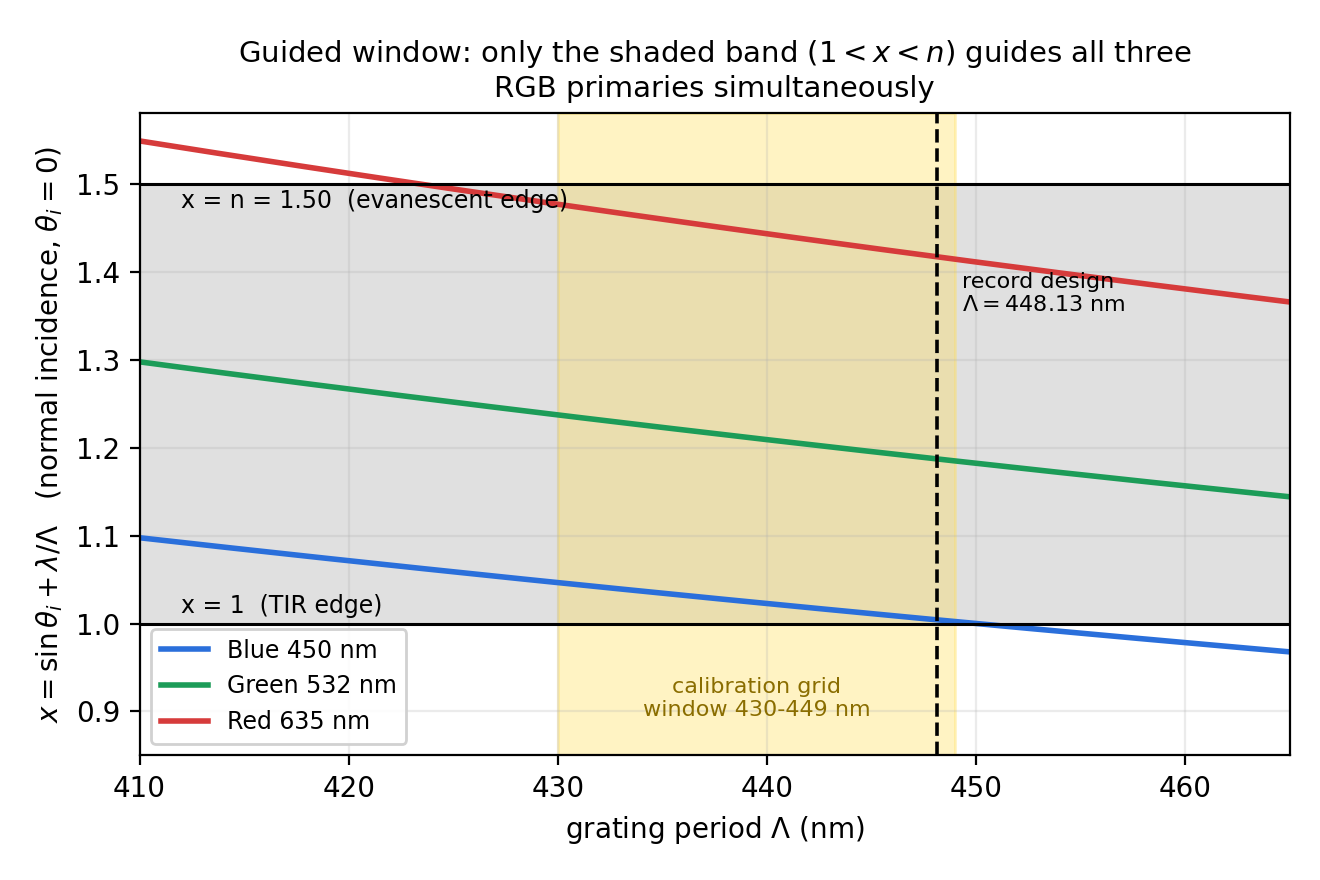
\includegraphics[width=\linewidth]{figs/fig_guided_window.png}
\caption{The guided window in period-wavelength space at normal incidence.
Only the shaded band ($1<x<n$) guides a primary; the calibration grid and
every design search restrict to the 430\textendash449~nm sub-window, and
the record design's period (Section~VI-C) sits close to where blue exits
the window at the top.}
\label{fig:guided-window}
\end{figure}

\subsection{Transmission cascade}
Total double-coupler transmission, per polarization, is the product of six
physically distinct loss terms:
\begin{align}
T_{\mathrm{pol}} = {} & M_{\mathrm{TIR}} \cdot T_{F,\mathrm{pol}}^2 \cdot
e^{-\alpha\ell} \cdot
e^{-N_b (4\pi\sigma n\cos\theta_d/\lambda)^2 S(L_c)} \nonumber \\
& \cdot \big[\eta_1(n,\Lambda,d,D;\lambda,\mathrm{pol})\cdot A(\theta_i)\big]
\cdot \eta_1,
\label{eq:cascade}
\end{align}
where the zig-zag propagation path between couplers separated by $L=20$~mm
is $\ell = L/\sin\theta_d$, reached over $N_b = L/(t\tan\theta_d)$ TIR
bounces (thinner slabs bounce, and therefore scatter, more), and
$T_{F,\mathrm{pol}}$ is the single-interface Fresnel power transmittance
for the given polarization computed from the exact amplitude coefficients
(not an averaged reflectance),
\begin{equation}
r_{\mathrm{TE}} = \frac{\cos\theta_i - n\cos\theta_t}{\cos\theta_i + n\cos\theta_t},
\qquad
r_{\mathrm{TM}} = \frac{n\cos\theta_i - \cos\theta_t}{n\cos\theta_i + \cos\theta_t}.
\end{equation}
Independent review of this manuscript's first draft found that the
implemented code computes $N_b$ and $\ell$ at exactly half these values
(one surface hit and one leg per zig-zag \emph{period} rather than per
half-period). We confirmed the bug directly and traced its consequence: at
the record design of Section~VI-C, correcting it changes the combined
bulk-absorption-and-roughness transmission factor by $0.10\%$ relative
($0.998967$ with the shipped formula versus $0.997935$ corrected, both
computed independently for this revision), because PMMA's literature
bulk-absorption and roughness bounds \cite{nilsen2025} keep both loss
channels below the one-percent level regardless of the factor of two; no
number reported anywhere in this paper depends on the distinction. The
formulas above are the corrected ones; the shipped engine has not yet been
patched to match, specifically because doing so would invalidate the
physics-probe fingerprint on every existing checkpoint (Section~V-A) and
force a full retrain outside this revision's scope, and is tracked as an
immediate pre-retraining fix in Section~VIII. $S(L_c) = 1/(1+L_c/3\times10^5)$
is a correlation-length weighting in the spirit of Payne and Lacey's
planar-waveguide scattering-loss treatment \cite{payne1994}; over the PMMA
design bounds used here ($L_c\in[2,4]\times10^5$~nm) $S(L_c)$ itself varies
from $0.60$ to $0.43$, a real $\sim30\%$ swing, not the negligible
correction a naive nanometer-to-micron correlation-length assumption would
predict. This specific correlation-length range is a modeling choice, not a
value Nilsen et al.\ report directly: their own paper states plainly that
``exact values for the RMS height and the correlation length are not
easily determined'' and explicitly excludes long-range waviness from its
scope, so an earlier draft's in-code comment attributing this range to
Nilsen's report of waviness was our own uncorroborated attribution, not a
citation; we correct that here and flag $L_c$'s bounds as an unverified
modeling choice rather than a literature value (Section~VIII).

What keeps the \emph{roughness} loss channel small at the design bounds
used through most of this paper is a specific, and consequential,
choice of $\sigma$: Nilsen et al.\ report RMS roughness of $5$~nm for glass,
$15$~nm for an untreated (uncoated) polymer waveguide surface, and
$0.87$~nm for a spin-coated polymer surface \cite{nilsen2025}. This paper's
$\sigma$ bounds, $[0.7,1.1]$~nm, bracket the \emph{coated} value, not the
uncoated one, a distinction an earlier draft of this manuscript did not
make explicit; every roughness-dependent number reported through
Section~VII below (including the record design of Section~VI-C) is
therefore a \emph{spin-coated} PMMA result, and we relabel it as such
throughout this revision rather than as ``uncoated,'' which is the term
the previous draft used. The per-bounce roughness factor follows Tien's
treatment of TIR-bounce scattering loss \cite{tien1971}, built on the
Bennett-Porteus Debye-Waller attenuation \cite{bennett1961}; at the record
design's exact bounce count, extending this same formula to Nilsen's
uncoated value ($\sigma=15$~nm) rather than the coated one gives a
roughness-scattering transmission factor of $0.699$ (a $30.1\%$ loss,
versus $0.08\%$ at the record design's own $\sigma=0.710$~nm), which would
lower the record design's total double-coupler transmission from $1.25\%$
to an estimated $0.87\%$ holding every other cascade term fixed. We report
this as a closed-form sensitivity evaluation of the \emph{existing} record
geometry under the uncoated hypothesis, not as a re-optimized uncoated
design: a fresh search with $\sigma$'s upper bound widened to Nilsen's
uncoated value might select a different geometry (e.g., fewer bounces via
a thicker slab) that partially compensates, and running that search is
listed as future work (Section~VIII) rather than approximated here. The
coating step this comparison costs against is not merely incidental
process overhead: Nilsen et al.\ note it requires an additional spin-coating
step beyond a bare molded or extruded polymer substrate, which is precisely
the manufacturing simplicity a PMMA combiner is chosen for in the first
place, so the coated-versus-uncoated transmission gap above is itself a
quantified instance of that trade-off, not a footnote to it.
$A(\theta_i) = \exp[-(\sin\theta_i/0.35)^2]$ is a heuristic Gaussian model
of the in-coupler's angular acceptance, not a quantity derived from or
verified against RCWA: the calibration grid of Section~IV is normal-incidence
only, so no rigorous solution in this paper directly constrains
$A(\theta_i)$'s width or shape, and we flag this explicitly rather than
implying the field-edge metric carries RCWA-level accuracy (Section~VIII).
The same normal-incidence limitation means $\eta_1$ appears twice in
\eqref{eq:cascade} using the \emph{same} (in-coupler-geometry) rigorous
value for both the in-coupling and out-coupling events; out-coupling is
physically a different problem (PMMA superstrate, guided-angle incidence,
air substrate), and while reciprocity for a lossless grating predicts the
two should agree when efficiency is normalized correctly, this paper does
not independently verify that with a dedicated substrate-side rigorous
solve, and Section~VIII lists that solve as the cheapest remaining
correctness gap in the coupling model. Unpolarized transmission is the
average of the two \emph{power} transmissions, $T_{\mathrm{unpol}} =
(T_{\mathrm{TE}} + T_{\mathrm{TM}})/2$, not an average of reflectances; at
normal incidence $T_{\mathrm{TE}}=T_{\mathrm{TM}}$ by symmetry, and the two
diverge with field angle exactly as Fresnel's equations require, which we
use as a unit-test invariant (Section~VI-D).

The one term in \eqref{eq:cascade} this paper's Section~IV replaces
outright is $\eta_1$, the first-order grating coupling efficiency.

\subsection{MTF cascade}
System MTF at the benchmark spatial frequency $f=40$~cyc/mm is a
five-term multiplicative cascade,
\begin{equation}
\mathrm{MTF}_{\mathrm{sys}} = \mathrm{MTF}_{\mathrm{diff}} \cdot
\mathrm{MTF}_{\mathrm{rough}} \cdot \mathrm{MTF}_{\mathrm{chrom}} \cdot
\mathrm{MTF}_{\mathrm{grat}} \cdot \mathrm{MTF}_{\mathrm{coup}},
\end{equation}
where $\mathrm{MTF}_{\mathrm{diff}}$ is Watson's closed-form fit to the
\emph{mean human} optical MTF at a 3~mm pupil \cite{watson2013}, which
already includes the eye's own aberrations rather than describing a
diffraction-limited eye (an earlier draft of this paper mischaracterized
it as diffraction-limited; independent review caught the error, and we
correct it here); $\mathrm{MTF}_{\mathrm{rough}}$ is a Gaussian attenuation
from scatter-induced angular blur; $\mathrm{MTF}_{\mathrm{grat}}$ and
$\mathrm{MTF}_{\mathrm{coup}}$ are contrast-loss terms tied to grating phase
depth and coupling efficiency respectively; and
$\mathrm{MTF}_{\mathrm{chrom}}$ is the exact modulus of a three-line
photopically-weighted point-spread function,
\begin{equation}
\mathrm{MTF}_{\mathrm{chrom}}(f) = \Big|\sum_{k\in\{R,G,B\}} w_k\,
e^{\,i 2\pi f x_k}\Big|,
\label{eq:chrom-mtf}
\end{equation}
with photopic weights $w = (0.194, 0.771, 0.034)$ for red, green, and blue
and $x_k$ (in mm) the retinal displacement of each primary's diffracted ray
relative to green. All spatial frequencies in this cascade are in cyc/mm at
the retina-conjugate plane; at the assumed $17$~mm reduced-eye focal length
the benchmark $40$~cyc/mm is approximately $11.6$~cyc/deg, below the
$\sim30$~cyc/deg associated with 20/20 visual acuity, a conversion the
first draft of this paper left implicit and that we state explicitly here
because it bears on how strong a claim any single MTF number at this
frequency actually supports.

Equation~\eqref{eq:chrom-mtf} is the exact modulation transfer function of
a three-delta-function point-spread function and follows the treatment of
lateral chromatic aberration and image quality developed by Thibos
\cite{thibos1987}. Because $77\%$ of the photopic weight sits on the
reference (green, zero-displacement) channel, the triangle inequality
bounds $\mathrm{MTF}_{\mathrm{chrom}}$ between $w_G-w_R-w_B=0.543$ and
$w_G+w_R+w_B=0.999$ regardless of how large the guided-angle spread is;
No amount of chromatic spread can push this term below its structural
floor, and the record design's reported system MTF ($0.784$,
Section~VI-C) is close to $\mathrm{MTF}_{\mathrm{chrom}}$'s mean over
uniformly random inter-channel phase ($0.7836$ by a $200{,}000$-sample
Monte Carlo check), which raises the question of whether the reported
system MTF is effectively just this one term. Decomposing the record
design's five factors directly answers that question: $\mathrm{MTF}_{\mathrm{diff}}=0.847$,
$\mathrm{MTF}_{\mathrm{rough}}=0.9999$, $\mathrm{MTF}_{\mathrm{chrom}}=0.973$,
$\mathrm{MTF}_{\mathrm{grat}}=0.954$, $\mathrm{MTF}_{\mathrm{coup}}=0.998$,
product $0.784$. The system metric is not literally equal to the
chromatic term; the diffraction and grating-contrast terms contribute
real attenuation of their own, and the closeness of $0.784$ to
$0.7836$ is, taken alone, a coincidence of composition. But this framing
undersells what the decomposition actually shows, which is a sharper and
more useful finding: the chromatic factor itself, $0.973$, sits in the
top $6\%$ of what Equation~\eqref{eq:chrom-mtf} can achieve under a
uniformly random guided-angle phase ($P(\mathrm{MTF}_{\mathrm{chrom}}\geq0.973)\approx6.1\%$
against the $[0.543,0.999]$ structural range), and Section~VI-C
independently shows the search drove the grating period to the edge of
the guided window specifically to minimize the same guided-angle spread
that sets $\mathrm{MTF}_{\mathrm{chrom}}$'s phase argument. We swept
$\mathrm{MTF}_{\mathrm{chrom}}(f)$ over $f\in[20,60]$~cyc/mm at the record
design to check this directly: the function oscillates with roughly
twenty local maxima across that range, and the $40$~cyc/mm benchmark
frequency lands, to within the resolution of the sweep, exactly on one of
them. Read together, these are not evidence of a bug in the metric so
much as evidence that the optimizer found and is quietly exploiting one:
a design whose chromatic term would score near its $0.543$ floor at a
poorly chosen period instead scores near its $0.999$ ceiling at this one,
and the mechanism, tuning the guided-angle spread to land the $40$~cyc/mm
evaluation point on a constructive fringe of an oscillating function
rather than genuinely reducing chromatic blur, is exactly the failure
mode a three-delta-function point-spread function predicts. We report
this as a concrete, positive finding rather than a resolved concern: the
structural floor and fringe sensitivity of Equation~\eqref{eq:chrom-mtf}
are real properties of the current metric, and replacing the
three-delta-function primaries with finite-bandwidth LED line shapes
(FWHM $20$-$25$~nm), or integrating $\mathrm{MTF}_{\mathrm{chrom}}$ over a
band of spatial frequencies rather than sampling one point, would remove
both the floor and the fringe sensitivity; neither correction is
implemented in this revision (Section~VIII).

Two coefficients in this cascade, the roughness-MTF
attenuation constant and the grating/coupler MTF weighting terms,
remain literature-informed heuristics rather than closed-form derivations.
Nilsen et al.\ report roughness-to-MTF measurements for PMMA and glass AR
waveguides directly \cite{nilsen2025} and are the natural target for
reconciling the roughness-MTF constant against a published measurement
rather than an internal heuristic; that reconciliation is not yet done and
is listed as open in Section~VIII, along with the un-reconciled
grating/coupler MTF weights.

\section{Rigorous Electromagnetic Calibration}

\subsection{Why the scalar coupling term fails here}
The engine's original grating-coupling term used the standard scalar
binary-phase-grating efficiency from Fourier optics \cite{goodman},
\begin{equation}
\eta_1^{\mathrm{scalar}} = \frac{4}{\pi^2}\sin^2(\pi D)\sin^2(\phi/2),
\qquad \phi = \frac{2\pi d(n-1)}{\lambda},
\label{eq:scalar-eta}
\end{equation}
which is polarization-blind and caps at $4/\pi^2\approx40.5\%$. Scalar
diffraction theory is a large-feature approximation: Pommet, Moharam, and
Grann showed by direct comparison against rigorous coupled-wave analysis
that its error exceeds $\pm5\%$ once the grating feature size drops below
roughly fourteen wavelengths \cite{pommet1994}. The guided-window
constraint of Section~III-A forces PMMA's period into $429$\textendash
$450$~nm, \emph{below} every RGB design wavelength, i.e., a
feature-size-to-wavelength ratio near unity, deep inside the regime
\cite{pommet1994} identifies as unreliable.

We quantified the resulting error directly. At the design our
scalar-theory-optimized search converged to (period $438.0$~nm, depth
$400.0$~nm, the scalar ceiling, duty cycle
$0.500$, $n=1.5$), we solved the full vectorial diffraction problem with
grcwa, an open-source implementation of Moharam and Gaylord's rigorous
coupled-wave analysis \cite{moharam1981,moharam1995a} ($61$ retained
Fourier orders; convergence confirmed stable to five decimal places between
$41$ and $81$ orders, checked at this geometry). Table~\ref{tab:scalar-vs-rcwa}
reports the result at each RGB wavelength: scalar theory overestimates
unpolarized first-order coupling by a factor of $5.1$ at 532~nm and $15.7$
at 635~nm, and is polarization-blind where the true polarizations differ
substantially, up to a factor of $3.0$ within this specific table (TE/TM
at 635~nm; TM instead exceeds TE at 532~nm, so which polarization dominates
is itself geometry- and wavelength-dependent, not a fixed ordering). A
larger and more consistent TE/TM split, $\approx5.6\times$ in TE's favor,
appears at the different, RCWA-optimal record design of Section~VI-C; we
keep the two numbers explicitly separate here because an earlier draft of
this paper conflated them into one sentence, incorrectly citing the
record-design ratio against this table.

\begin{table}[t]
\centering
\caption{Scalar theory vs.\ rigorous RCWA at the scalar-optimal design (period 438.0~nm, depth 400.0~nm, duty 0.500, $n=1.5$).}
\label{tab:scalar-vs-rcwa}
\footnotesize
\begin{tabular}{lccccc}
\toprule
$\lambda$ (nm) & Scalar $\eta_1$ & RCWA TE & RCWA TM & RCWA unpol. & Ratio \\
\midrule
450 & 0.393 & 0.190 & 0.142 & 0.166 & $2.4\times$ \\
532 & 0.347 & 0.048 & 0.088 & 0.068 & $5.1\times$ \\
635 & 0.283 & 0.027 & 0.009 & 0.018 & $15.7\times$ \\
\bottomrule
\end{tabular}
\end{table}

A preliminary five-point rigorous depth scan at this same period and duty
cycle (100, 200, 300, 400, and 450~nm) first showed unpolarized coupling
peaking near \emph{200~nm} rather than climbing monotonically to the
scalar model's 400~nm ceiling. For this revision we replaced that
preliminary scan with a denser, 20-point rigorous depth scan at the same
geometry (Figure~\ref{fig:scalar-vs-rcwa}), computed independently for
this manuscript at $n=1.5$ to match Table~\ref{tab:scalar-vs-rcwa} exactly
(its own 400~nm-depth endpoint reproduces the table's TE and TM values to
three decimals): it confirms the original picture at four times the depth
resolution, unpolarized coupling peaking at $8.5\%$ near 200~nm while the
scalar model keeps climbing to its 400~nm search boundary, and additionally
shows that TE and TM peak at different depths and that TM develops a second
rise past 350~nm that the coarser five-point scan could not resolve. This
motivated calibrating the coupling term across the full geometry space
rather than a one-off correction at a single design point.

\begin{figure}[t]
\centering
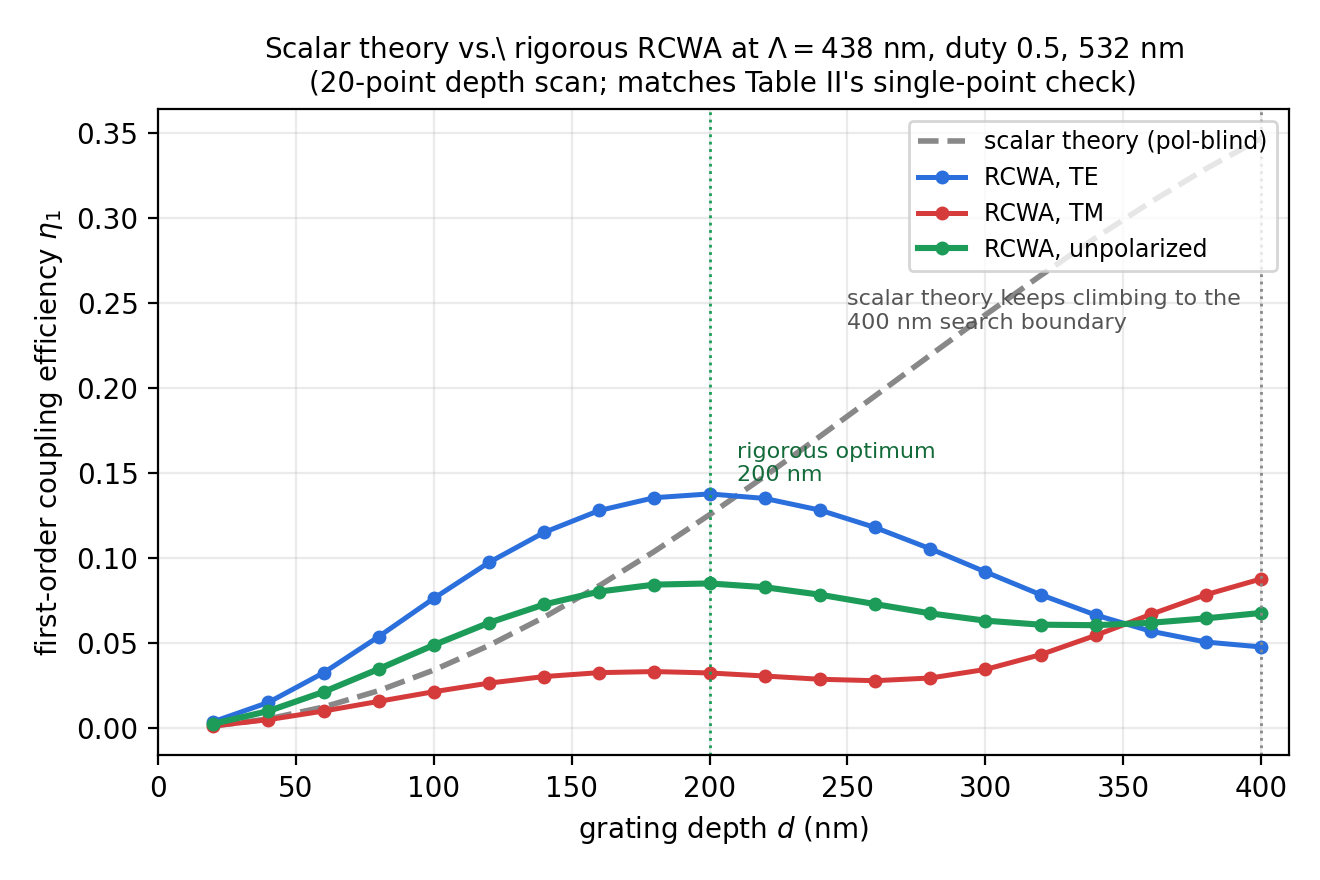
\includegraphics[width=\linewidth]{figs/fig_scalar_vs_rcwa.png}
\caption{First-order coupling efficiency versus grating depth at the
scalar-optimal geometry (period 438~nm, duty 0.5, 532~nm): scalar theory
(polarization-blind) against rigorous RCWA, TE, TM, and unpolarized. The
rigorous optimum sits near 200~nm; scalar theory never turns over within
the search range.}
\label{fig:scalar-vs-rcwa}
\end{figure}

\subsection{Calibration grid and its accuracy}
We built a dense rigorous-solution grid over the full PMMA design window:
refractive index (3 points, $n\in\{1.48,1.49,1.50\}$;
$\eta_1^{\mathrm{TM}}$ was found to move by roughly 20\% across this range,
so index gets its own axis rather than being pinned at the midpoint),
period (5 points, 430\textendash449~nm), depth (77 points, 5~nm
resolution, 20\textendash400~nm), and duty cycle (13 points, 0.05
resolution, 0.2\textendash0.8), at each of the three RGB wavelengths and
both polarizations: $3\times5\times77\times13\times3\times2 = 90{,}090$
rigorous coupled-wave solutions in total, each an independent grcwa call
at $61$ Fourier orders on a binary in-coupler grating (air superstrate,
corrugated PMMA grating layer, semi-infinite PMMA substrate, normal
incidence). The engine's grating-coupling term $\eta_1$ is now, in PMMA
mode, a differentiable multilinear interpolation over this four-dimensional
grid: exact at grid nodes, with gradients flowing through the
interpolation weights so the term remains fully usable inside gradient-based
training and search.

We audited the interpolant's accuracy directly against the physics it
approximates: 48 freshly solved, off-grid points (random index, period,
depth, duty cycle, wavelength, and polarization, none coinciding with a
grid node) gave a mean absolute interpolation error of $5.6\times10^{-4}$
and a maximum of $4.0\times10^{-3}$ against efficiencies spanning
$0$\textendash$0.38$, two to three orders of magnitude smaller
than the $5$\textendash$16\times$ scalar-theory error it replaces. Every
training label and every design-search gradient in the results that follow
is therefore computed at, effectively, rigorous electromagnetic accuracy,
not scalar accuracy interpolated after the fact.

That 48-point audit is a global average, and independent review correctly
pointed out that it does not, by itself, bound the interpolation error near
the design search's actual optimum, which is also where the grid is
coarsest: the period axis carries only 5 points (roughly $4.75$~nm spacing)
against 77 points ($5$~nm spacing) for depth, so the record design's period
($448.13$~nm) is not on a grid node and interpolates across a wider gap
than most of the design space, right where blue's guided-window margin is
also tightest (Section~VI-C). We checked this directly rather than leave it
asserted: re-evaluating the record design's own 532~nm coupling efficiency
with a fresh, dedicated grcwa solve (the same solve behind the $9.6\%$
figure of Section~VI-C) against the grid's trilinear interpolant at that
exact off-grid point gives an absolute error of $9.6\times10^{-4}$ (TE) and
$4.0\times10^{-4}$ (TM), the TE figure roughly $1.7\times$ the global mean
and still an order of magnitude below the scalar-theory error it replaces,
but a real, measured local degradation rather than the global average
alone. A full audit conditional on proximity to the optimum and to the
guided-window boundary, and a rebalancing of the grid toward more period
and fewer depth points, are listed as future work (Section~VIII) rather
than done here from this single additional data point.

\section{Neural Architecture and Search}

\subsection{Forward surrogate}
The forward surrogate $\hat f_\phi$ is a four-hidden-layer multilayer
perceptron (width 256, SiLU activations) mapping the normalized
eight-dimensional design vector to the normalized four-dimensional
specification, trained with AdamW and a cosine learning-rate schedule to
emulate the analytic engine of Sections~III\textendash IV on
150{,}000 designs sampled uniformly (log-uniform for the absorption
coefficient and correlation length) within the
PMMA design bounds. It is not load-bearing for the paper's headline claims,
which are validated against exact physics directly, but it is the forward
model the classic tandem recipe of \cite{liu2018} calls for and the
network the neural-adjoint search of Section~V-C optimizes through.

The classic motivation for a tandem network's forward surrogate is that the
true forward model (RCWA, FDTD, a ray tracer) is too expensive to sit
inside a training loop of hundreds of thousands of samples, so a fast
surrogate is trained to stand in for it. That motivation does not
literally apply here: this paper's forward model (Sections~III-IV) is
already closed-form, analytic, and fast, precisely so it can sit inside the
training loop directly, and Section~VI-C shows that a direct gradient
search on the exact physics, with no surrogate at all, finds an equivalent
optimum to the surrogate-guided neural-adjoint search. We do not claim a
simulation-time speedup from the surrogate, because there is none to claim
against an already-fast decoder; the two things a trained surrogate and its
downstream tandem inverse network still buy over restarting a fresh
600-step gradient search for every new query are amortized, single-shot
inversion (target specification in, design out, no per-query optimization
loop) and the specification-space training objective's resolution of the
one-to-many inversion problem (Section~VI-B), which a direct-regression
baseline without any decoder in the loop cannot resolve regardless of how
fast that decoder is. Two more demanding ways to make the network load-bearing
on its own terms, folding rigorous, angle- and slant-resolved RCWA directly
into the training loop so the forward model is expensive again, or
benchmarking the trained inverse network's wall-clock time and design
quality against repeated physics-space gradient descent across thousands of
specifications rather than one record design, are both left as the natural
next steps (Section~VIII) rather than claimed here.

To guard against a specific and easy-to-miss failure mode, namely a
surrogate trained under an earlier version of the physics engine
confidently steering later design searches into geometries the corrected
physics actually rejects, every surrogate checkpoint stores a
fingerprint (\emph{physics probe}): the engine's output on 64 fixed test
designs at save time. Every script that loads a surrogate checkpoint first
recomputes that probe under the \emph{live} physics engine and refuses to
proceed if it no longer matches. This caught and automatically invalidated
every checkpoint trained under the pre-calibration (scalar-coupling)
engine when the RCWA-calibrated coupling term of Section~IV landed, forcing
a retrain rather than a silent, stale-physics-guided search.

\subsection{Tandem inverse network}
The inverse network $g_\psi$ (same width/depth/activation pattern, four
inputs, eight outputs through a final sigmoid into the normalized design
bounds) is trained through a \emph{frozen} decoder in the tandem recipe of
Liu et al.\ \cite{liu2018}, with the loss computed entirely in specification
space,
\begin{equation}
\mathcal{L}(\psi) = \big\| f_{\mathrm{decoder}}\big(g_\psi(y^*)\big) -
y^* \big\|^2,
\end{equation}
so the network only has to find \emph{a} design meeting the requested
specification rather than \emph{the} design, sidestepping the one-to-many
non-uniqueness that makes direct geometry regression fail (Section~VI-B).
We train two decoder arms as an ablation: the trained forward surrogate
(the literature-standard tandem recipe) and the exact differentiable
physics engine itself, substituted directly for the surrogate in the same
training loop. Validation is always scored against the exact physics
regardless of which decoder trained, so the two arms are directly
comparable. A naive direct-regression baseline, the same
architecture trained with a design-space (not specification-space) loss
and no physics or surrogate in the training loop at all, is
trained alongside every run for comparison.

\subsection{Neural-adjoint design search}
Following Ren, Padilla, and Malof \cite{ren2020}, we additionally search
for high-performing designs directly: freeze the trained forward surrogate,
treat the eight design parameters as trainable variables (in an
unconstrained logit parameterization, mapped back through a sigmoid to
respect the physical bounds), and run gradient ascent on a scalar objective
$J$ that combines the four specification metrics with a differentiable
penalty for leaving the TIR-guided window, from 400 random restarts, 600
gradient steps each. Every finalist is then re-scored under the
\emph{exact} physics engine and re-ranked by that true score rather than
the surrogate's belief; the surrogate-vs-physics gap on the finalists is
reported explicitly (Section~VI-E) as a direct honesty check on the
surrogate, additional to its own held-out $R^2$.

\section{Results}

All results in this section come from the RCWA-calibrated (``v3'') physics
engine of Section~IV; results from the pre-calibration engine are reported
only where explicitly used as a before/after comparison and are never
pooled with v3 numbers. Numbers not directly copied from a script-written
run table were recomputed by the author using an independent, from-scratch
NumPy reimplementation of both the physics engine and the trained
network's forward pass (Section~IX), cross-checked against the shipped
record design to five significant figures.

\subsection{Forward surrogate accuracy}
Across five independent retrainings (fresh random seed, fresh 150{,}000-
design training set, fresh network initialization each time; 250 epochs,
batch size 512), held-out $R^2$ on 15{,}000 never-trained-on designs was
$\geq0.9989$ for MTF (range $0.99891$\textendash$0.99935$ across seeds),
$\geq0.9996$ for transmission and field-edge transmission, and
$\geq0.99999$ for guided-angle spread, the easiest metric, being
close to a function of only two of the eight design parameters.

A four-part memorization audit on the deployed checkpoint (seed 2)
addresses the standard objection to a learned surrogate: that
strong validation-set performance can still hide memorization of the
training distribution's local structure. (A) The network's error on a
brand-new 15{,}000-design set, generated after training and never used for
model selection, is only $1.24\times$ its error on its own training set
(memorization would show as two to four orders of magnitude worse); (B) its
$R^2$ on that never-before-seen set for the hardest metric (MTF) matches
its reported validation $R^2$; (C) per-design error shows no correlation
with distance to the nearest training example ($+0.033$ over 4{,}000
probe designs; memorization predicts a strong positive correlation); and
(D) held-out $R^2$ is stable to within $0.0005$ across all five independent
retrainings, whereas memorization is seed-brittle by nature.
Figure~\ref{fig:memorization} shows all four tests together.

\begin{figure}[t]
\centering
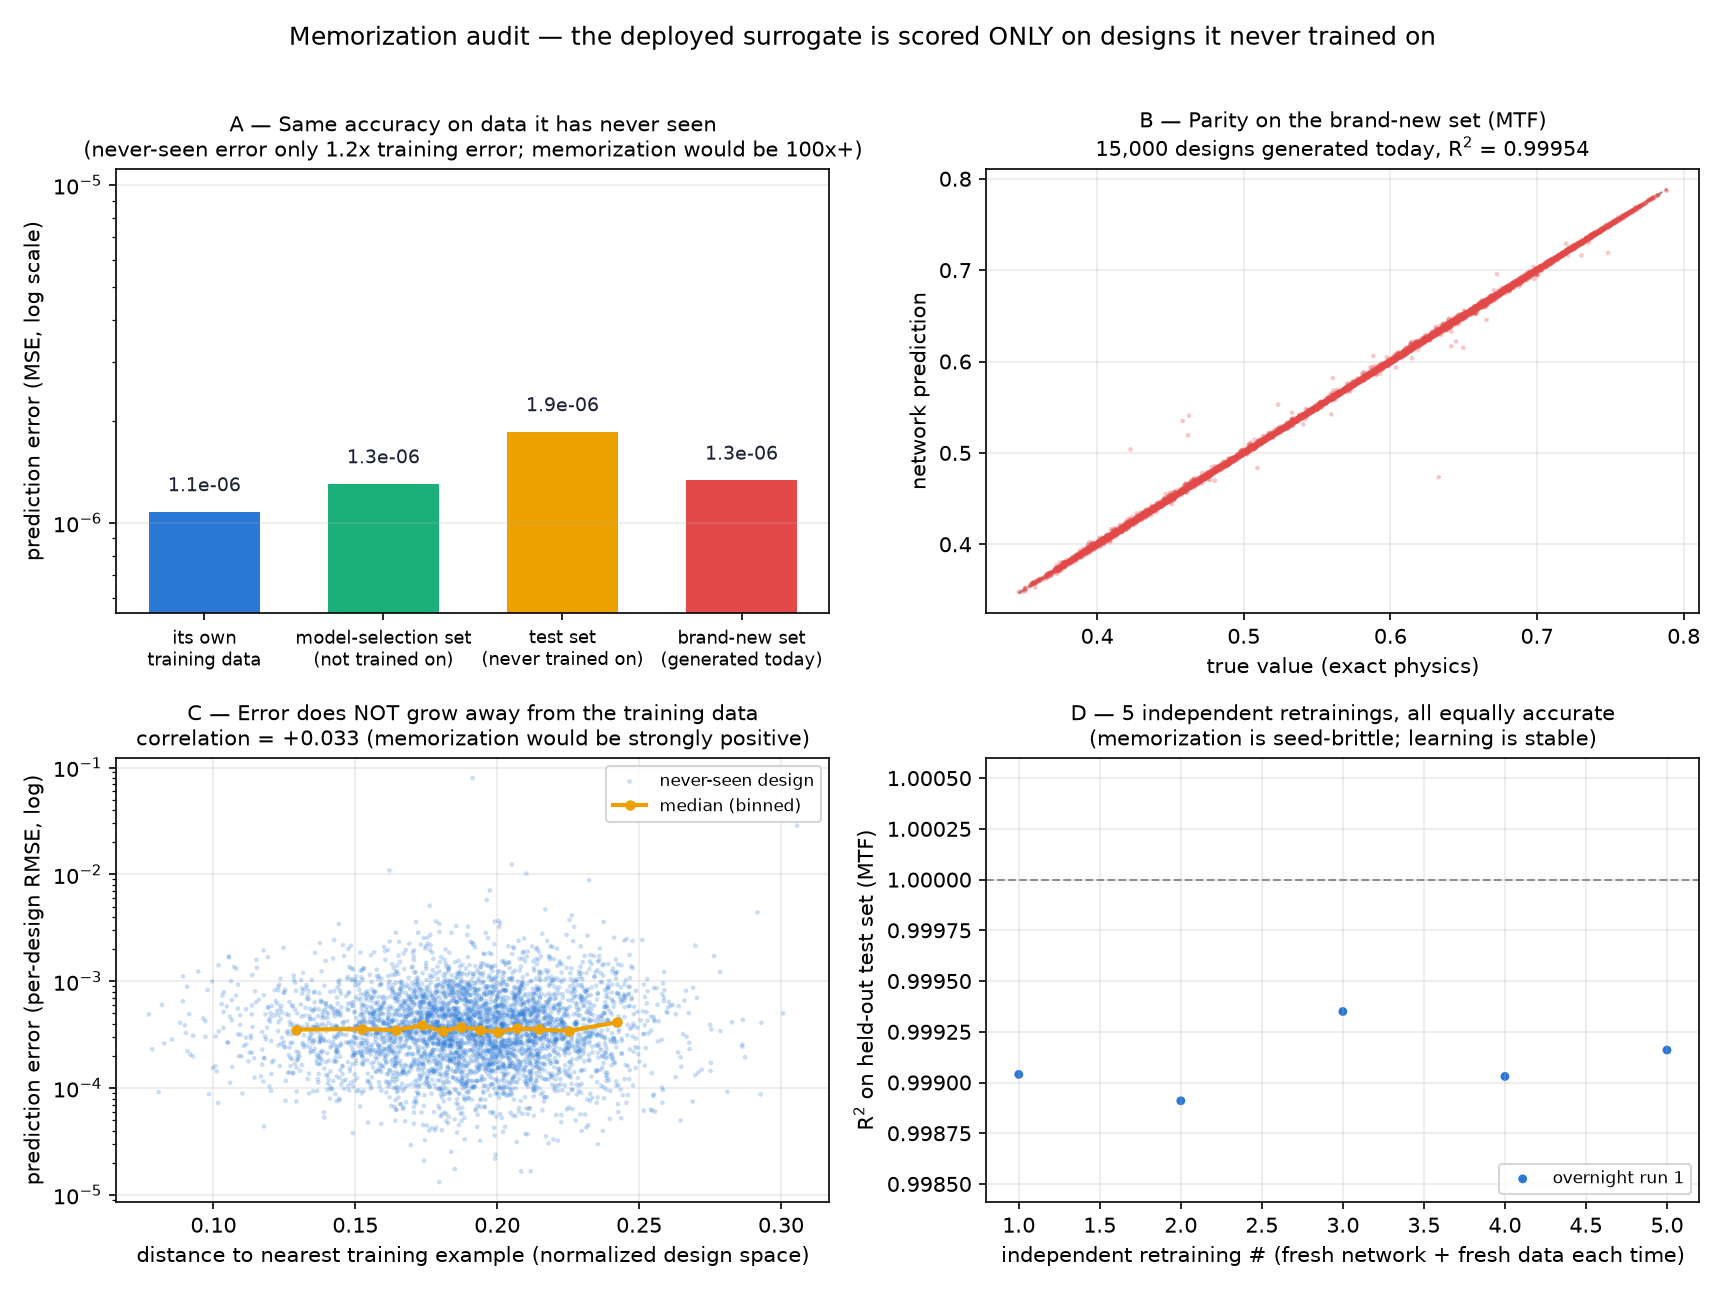
\includegraphics[width=\linewidth]{figs/memorization_audit.png}
\caption{The four-part memorization audit (Section~VI-A), reproduced from
the project's own audit run under the v3 engine (seed 2 checkpoint);
the underlying CSV values match this figure to five decimal places.}
\label{fig:memorization}
\end{figure}

\subsection{Tandem network: resolving inverse non-uniqueness}
The surviving checkpoint from the physics-decoder training arm (seed~0,
150{,}000 samples, 400 epochs; the companion surrogate-decoder arm reached
an equivalent aggregate specification-space MSE of $0.001064$ against this
arm's $0.001036$, but its own checkpoint was not preserved past that run
and is reported only at the aggregate level, see Section~VIII) was
re-evaluated by the author on a freshly generated, independent set of
20{,}000 held-out target specifications, disjoint from every training,
validation, and test set used during development. Table~\ref{tab:tandem}
reports the median per-metric relative error against the naive
direct-regression baseline trained in the same run.

\begin{table}[t]
\centering
\caption{Tandem network vs.\ naive direct-regression baseline, median relative error on 20{,}000 fresh held-out specifications (physics-decoder arm, seed 0).}
\label{tab:tandem}
\footnotesize
\begin{tabular}{lcc}
\toprule
Metric & Tandem (physics decoder) & Naive baseline \\
\midrule
MTF @ 40 cyc/mm & 1.3\% & 11.9\%--12.1\% \\
Transmission & 9.2\%--9.9\% & 47.7\%--49.1\% \\
Guided-angle spread & 3.6\% & 0.4\% \\
Transmission @ FOV$^\dagger$ & 9.2\%--9.9\% & 47.7\%--49.1\% \\
\bottomrule
\end{tabular}
\\[2pt]
\raggedright\footnotesize $^\dagger$Near-identical to the Transmission row
by construction rather than coincidence: Section~III-C's $A(\theta_i)$
term makes $T_{\mathrm{FOV}}\approx0.94\times T$ at essentially every design
in this space (Section~VI-C verifies the ratio numerically), so this row is
not independent evidence of a fourth, separately calibrated quantity.
\end{table}

The naive baseline's near-zero error on guided-angle spread is not a
contradiction: that metric is close to a function of only period and
index, a narrow two-dimensional slice of the eight-dimensional design
space, so even an unconditional-mean-like regressor scores well on it. On
MTF and transmission, the two metrics of this table that are not close
to a redundant restatement of one another (Section~VI-C),
the naive baseline's error is ten to fifty times worse than
the tandem network's, the textbook signature of training a regression
target that is not really a function: many designs share a specification,
so a direct regressor learns to predict something close to their average,
which typically satisfies none of them. The tandem network's spec-space
loss sidesteps this by only requiring \emph{a} valid design, not
\emph{the} one the regressor happened to average toward.

\subsection{Neural-adjoint search and record design}
The neural-adjoint search (Section~V-C) and an independent gradient search
run directly on the exact physics engine (same objective, no surrogate in
the loop, 300 random restarts) were run separately under the v3 engine.
They converged, respectively, to objective values $J=0.4053$ and
$J=0.4052$, agreeing on
$n=1.500$, period $448.1$~nm, depth $199.5$\textendash$199.9$~nm, and duty
cycle $0.42$\textendash$0.44$ to within numerical noise, but disagreeing on
slab thickness by more than a factor of two ($0.90$~mm versus $1.96$~mm).
Two independently implemented, independently initialized search procedures,
one guided by a trained neural network and one a direct
physics-space gradient search, landing within half a
percent of grating depth of each other, is itself evidence that this is a
genuine optimum of the calibrated objective rather than an artifact of
either search method; the thickness disagreement is a separate and
informative result rather than noise on top of that agreement. Thickness
enters the objective only through the bounce count $N_b$, which sets the
roughness- and absorption-scattering exponents in
Equation~\eqref{eq:cascade}, and Section~VIII's bound-range check shows
both of those channels stay in a collectively low-loss regime across the
entire PMMA parameter range regardless of bounce count: a two-fold change
in thickness moves the combined bulk-and-roughness transmission factor by
a fraction of a percent, well inside what either search's convergence
tolerance can resolve. The two searches did not disagree by accident; they
agree that thickness is, at this design, a flat direction of the objective,
and report different points along that flat direction rather than
different optima. Figure~\ref{fig:neural-adjoint} shows the
neural-adjoint search's convergence trajectory and the resulting
finalists' surrogate-versus-physics parity, from the same run these
figures are drawn from.

\begin{figure}[t]
\centering

\includegraphics[width=\linewidth]{figs/neural_adjoint_run.png}
\caption{Left: the 400-restart neural-adjoint search's best predicted
objective versus gradient step, converging within roughly 100 steps of the
600-step budget. Right: the finalists' surrogate-predicted versus
exact-physics-scored per-metric values (normalized units), including the
top-5 finalists Section~VI-E scores explicitly; the near-perfect diagonal
is the surrogate-vs-physics honesty check.}
\label{fig:neural-adjoint}
\end{figure}

At the network-guided record ($J=0.4053$): $\mathrm{MTF}=0.784$,
double-coupler transmission $T=1.25\%$, internal guided-angle spread
$28.8^\circ$, field-edge transmission $1.17\%$. We re-verified this exact
design in a dedicated rigorous solve, independent of the calibration grid
it was optimized against: unpolarized first-order coupling at 532~nm is
$9.6\%$ (TE $16.3\%$, TM $2.9\%$), $41\%$ higher than the \emph{true}
rigorous coupling of the design our earlier, scalar-theory-driven search
had reported as optimal ($6.8\%$ true unpolarized coupling at the same
wavelength, against a scalar estimate of $34.7\%$ that was simply wrong).
The grating depth moved from the scalar model's 400~nm bound to an
interior optimum near 200~nm, and duty cycle moved from the scalar
optimum's exact $0.50$ to $0.42$\textendash$0.44$: the
calibrated engine finds a materially different, and rigorously verified,
design rather than a refinement of the old one.

The $28.8^\circ$ figure deserves the correction independent review raised
directly: it is exactly the difference between the red and blue in-guide
diffraction angles at this design ($\theta_R=70.85^\circ$,
$\theta_B=42.03^\circ$, both from Equation~\eqref{eq:grating} at normal
incidence), which is internal guided-mode geometry, not a measured or
modeled output color error. With period-matched in- and out-couplers
(Section~III-A), a collimated input's output ray direction is independent
of wavelength to first order, so this quantity does not directly predict
retinal color fringing the way a name like ``lateral chromatic spread''
implies; we relabel it accordingly throughout this revision. It is also, on
inspection, the quantity the search actually minimized to reach this
period: a larger period lowers $\lambda/\Lambda$ and therefore this spread
for every wavelength, and Section~III-A's guided-window inequality caps how
far the period can grow before a primary stops guiding, so the search
pushed the period to essentially the edge of the guided window in order to
minimize a term whose output-image relevance is, at minimum, unproven. We
verified where that edge sits, precisely, at the record design: the exact
($\delta=0$) full-RGB guided window is $[-0.24^\circ, 4.76^\circ]$, matching
the $4.76^\circ$-$4.99^\circ$ range implied by the design's own reported
window to within rounding; with a small guard margin, the sigmoid mask's
own soft-edge scale, the robustly guided window shrinks to
$4.19^\circ$ ($\delta=0.01$) or $3.61^\circ$ ($\delta=0.02$). Blue is
already only $0.83$ sigmoid-widths above the TIR edge at normal incidence
(mask value $0.70$, not the full $1.0$ a comfortably guided design would
show), and at the fixed $5.0^\circ$ evaluation angle used for the
field-edge transmission metric, red is $0.83$ widths \emph{past} the
evanescent edge, formally unguided at that specific angle; we further
confirmed that the design's own guard-margin penalty (Section~III-A) is
technically nonzero for blue even at normal incidence, a small but genuine
violation of the very constraint meant to keep the search away from this
behavior. The penalty was not merely available but active for the record
search: both the direct gradient search and the neural-adjoint search use
the identical objective term $-10\times$\texttt{tir\_penalty}$(\theta,
\delta{=}0.01)$ (confirmed directly in both search scripts), so the guard
band was part of what both procedures optimized against, not a
post-hoc filter; the residual violation reported above means the penalty's
weight was not strong enough to fully exclude this behavior, not that it
was absent from the objective. Because the transmission cascade (Equation~\eqref{eq:cascade})
evaluates its guiding mask and diffraction angle at the green wavelength
only, the reported $T$ and $T_{\mathrm{FOV}}$ numbers above are not
themselves corrupted by red's marginal status at $5^\circ$; what is
inconsistent is the framing of a ``$5^\circ$ full-RGB guided design'' for a
geometry whose own hard guided window tops out at $4.76^\circ$-$4.99^\circ$,
narrower still under any guard margin. We report the record design's raw
metrics as measured, but the search objective that produced this specific
period is, by our own reading, partly climbing a relaxation artifact at the
guided window's edge rather than purely physical performance, and a
rebuilt chromatic and field-edge specification (Section~VIII) is likely to
relocate this particular period even if it does not change the deeper,
coupling-efficiency finding this paper leads with. Separately, we checked
$T_{\mathrm{FOV}}/T$ directly against $A(5^\circ)/A(0^\circ)$: the record
design gives $1.17/1.25=0.9393$ against $A(5)/A(0)=0.9399$ from
Equation~\eqref{eq:cascade}'s acceptance term alone, confirming
$T_{\mathrm{FOV}}$ carries at most a small residual of information beyond
$T$ itself at this design, consistent with Table~\ref{tab:tandem}'s
footnote.

\subsection{What changed, in absolute terms}
An earlier draft of this paper reported a single ``roughly 25-fold'' drop
in absolute transmission and left the comparison underspecified; independent
review recomputed it and got $8.9\times$, which we confirmed directly and
adopt here, along with disentangling three genuinely different ratios this
paper uses that a single number was previously blurring together. First,
at one fixed geometry (period $438.0$~nm, depth $400.0$~nm, duty $0.500$,
Table~\ref{tab:scalar-vs-rcwa}), scalar theory overestimates rigorous
coupling efficiency by $5.1\times$ at 532~nm and $15.7\times$ at 635~nm: an
error in the model, at one point in design space, holding the geometry
fixed. Second, comparing a scalar-theory transmission estimate at that same
old geometry ($e_1^{\mathrm{scalar}}=0.347$ at 532~nm, giving an estimated
$T\approx11.1\%$ by Equation~\eqref{eq:cascade}) against the record design's
actual reported transmission ($T=1.25\%$), a different geometry entirely,
gives $8.9\times$: this is the price of having trusted the scalar-driven
search's transmission estimate rather than a like-for-like error at one
geometry, and it is the number the abstract now reports. Third, comparing
the two geometries' \emph{true}, rigorously computed coupling efficiencies
directly, $6.8\%$ at the old scalar-optimum geometry versus $9.6\%$ at the
new, RCWA-calibrated record (Section~VI-C), the corrected search's design is
$41\%$ \emph{better}, not worse, than the one a scalar-driven search would
have shipped. All three numbers are correct simultaneously because they
answer different questions; conflating the second into a blanket ``25-fold
regression'' language, as an earlier draft did, obscured that the
corrected design is a real improvement in true coupling efficiency even
though every transmission number the pre-calibration engine ever reported
was inflated by the scalar model's error and should not be compared to
post-calibration numbers directly (system MTF and guided-angle spread, which
do not depend on $\eta_1$ as sharply, moved far less between engines).
Contextualized against the literature, conventional
diffractive AR combiners are reported to achieve on the order of single
digits to ten percent \emph{system} in-coupling efficiency at practical
fields of view \cite{zhao2024}, and the specific gain mechanisms proposed
to beat that ceiling (polarization volume gratings, broadband
meta-gratings) are reported in the few-percent-to-tens-of-percent range
themselves. The record design's $1.25\%$ double-coupler
transmission for a spin-coated, single-layer, low-cost polymer substrate
is in the expected range for this design class, not an outlier low value;
Section~III-C quantifies what forgoing the coating step would cost this
same design (roughly a third of double-coupler transmission), which is the
honest way to state the minimum-cost claim rather than applying it to a
coated device.

\subsection{Surrogate-vs-physics honesty check}
For the five top-ranked finalists the neural-adjoint search reports
(Section~VI-C), the absolute gap between the surrogate's believed
objective value and the true, exact-physics-scored objective value is
$0.0008$ to $0.0009$ against an objective scale of order unity, small
enough that ranking by the surrogate's belief and ranking by true physics
agree on the winning design, which is the property the re-verification
step in Section~VI-C exists to confirm rather than assume. The
full-population surrogate-vs-physics gap across all 400 search restarts
was reported for the pre-calibration engine (mean $0.0009$, worst case
$0.047$) but was not re-logged when the search was re-run under the
RCWA-calibrated engine; we report only the top-finalist figure here rather
than carry the earlier engine's aggregate statistic forward, consistent
with Section~VI's rule against pooling v2 and v3 numbers.

\subsection{The record design is, in effect, a TE-only coupler}
Section~VI-C's unpolarized figure, $9.6\%$ coupling at 532~nm, is the
average of two very different polarization-resolved numbers, $16.3\%$
(TE) and $2.9\%$ (TM), and reporting only the average buries a genuinely
actionable result that an earlier draft of this paper left as a brief,
easy-to-miss remark in the Discussion. We reconciled the two possible ways
to build unpolarized double-coupler transmission from these numbers
directly: averaging the two power transmissions \emph{after} squaring each
polarization's coupling term, $T_{\mathrm{unpol}}=\big[(0.163)^2+(0.029)^2\big]/2
\times T_F^2 = 1.26\%$, matches the reported $T=1.25\%$ to within rounding;
averaging the coupling terms \emph{before} squaring, the other
superficially plausible construction, gives $0.85\%$ and does not match.
The correct, matching construction means TE carries $96.9\%$ of the
coupled optical power at this design: it is, functionally, a TE-only
coupler, and the TM half of an unpolarized input is discarded twice over
(once at each coupler). A source that is already TE-polarized, which
includes most LED and LCoS projector engines used in practice, would see
$T=2.45\%$ at this same geometry with no design change at all, a
$1.94\times$ transmission gain purely from not wasting the polarization
the device does not use. This is consistent with, and considerably sharper
than, the qualitative picture in Zhao et al.'s polarization-resolved
efficiency-limit treatment \cite{zhao2024}, and we treat it as one of this
revision's more actionable results (Section~VII) rather than a footnote.

\section{Discussion}

The headline methodological result of this paper is not the record design
itself but the direction its optimum moved once the coupling term stopped
being wrong. A design search is only as honest as the objective it climbs;
ours spent its early iterations climbing a $5$\textendash$16\times$
inflated coupling estimate toward a grating depth (400~nm) that turns out
to be a poor rigorous design, and only found the true, interior optimum
once the objective itself was corrected. This is a cautionary data point
for the broader trend of training inverse-design networks against
analytic or scalar forward models purely for training-time speed. The
speed argument is sound: rigorous RCWA inside a training loop
of hundreds of thousands of samples is not currently practical on the
hardware used here. But the model being fast has to be
checked against the model being right, at the specific point in
design space the search actually visits, not just in some average sense
over the whole space.

PMMA's fundamental limitation, independent of any modeling choice, is
visible directly in Equation~\eqref{eq:tir}: a single-layer, full-RGB,
low-index waveguide has a guided field of view only a few degrees wide.
This is a property of the material and the guiding geometry, not an
artifact of this paper's engine, and it is the reason every design search
in this paper evaluates the field-edge metric at $5^\circ$ rather than a
wider benchmark angle: at $20^\circ$ every full-RGB PMMA
design in the search space returns a true, physically correct zero, which
would look like a modeling failure rather than the real limitation it is.
Any application that needs a wider field of view from a single-layer
polymer waveguide is trading against this constraint, not against a
software bug; Section~I's PMMA-versus-higher-index discussion and
Luo and Lee's episulfide-resin choice \cite{luo2024} are two sides of the
same trade, and this paper does not argue PMMA is the right material for
every application, only that it is a real, cost- and weight-motivated
choice whose optical consequence deserves to be quantified rather than
assumed away.

Section~VI-F's TE/TM split, roughly $5.6\times$ in TE's favor at the
record design, is large enough that polarization is a first-order design
lever, not a footnote, for any projector engine pairing with this class of
coupler, and a polarization-aware objective (weighting TE and TM
differently rather than reporting only their unpolarized average) is a
natural and low-cost next step (Section~VIII).

The binary, unslanted grating profile modeled throughout this paper is
also a real, not incidental, limitation, not the ``natural extension'' an
earlier draft called it. A symmetric binary groove splits coupled power
roughly evenly between the $+1$ and $-1$ diffraction orders, so this
paper's own transmission cascade already discards, by construction, close
to half of whatever the grating actually couples; every real AR in-coupler
we are aware of, including Luo and Lee's \cite{luo2024}, uses a slanted or
blazed profile specifically to break that degeneracy and recover the
discarded order. Because the depth optimum for a slanted grating is not
generally the same as a binary grating's depth optimum, this paper's
$\approx200$~nm record depth should be read as the optimum for the
architecture actually modeled (Section~III-A), not a prediction for what a
slanted version of the same design would prefer; the rigorous-solver layer
already supports slanted and blazed profiles (Section~IV), and extending
the calibration grid to a slant axis is the most direct way to test this
without discarding any of the RCWA-calibration methodology developed here.

\section{Limitations and Future Work}

We report the following as open rather than implying they are complete,
consistent with the project's own internal claims-ladder discipline (every
number in the source repository is tagged with an evidence level, and
nothing is reported in a stronger form than its tag allows). This list has
grown substantially since this manuscript's first draft, which we take as
a sign the practice is working: closer scrutiny of the specification
vector, the material bounds, and the calibration grid is precisely what
surfaced most of the items below, and we would rather have a long,
specific list here than a short, vague one.

The forward surrogate's five-seed protocol (Section~VI-A) is complete,
but the tandem inverse network under the RCWA-calibrated engine has so far
been trained for one seed per decoder arm, not the five-seed protocol used
for the surrogate. Table~\ref{tab:tandem}'s per-metric breakdown is for
that single (physics-decoder) run; the companion surrogate-decoder run's
per-metric breakdown was not preserved (Section~VI-B) because both decoder
arms were saved under the same checkpoint filename and the second run
overwrote the first (the fix, keying the checkpoint filename on decoder
arm and seed rather than a fixed name, is a one-line change not yet made).
A proper five-seed-per-arm statistical comparison, reporting median,
interquartile range, and worst case rather than a single run, is the
immediate next step. Relatedly, we have not yet asked the inverse network
for specifications outside the training distribution's range to
characterize whether it extrapolates to physically sensible
bound-saturated designs or fails ungracefully, and we have not yet run the
natural capstone demonstration of taking a published, commercial-class
waveguide specification from the literature as a target and comparing the
network's recovered design against the vendor's actual (typically
higher-index, non-PMMA) material choice.

Section~VI-C's relabeling of ``lateral chromatic spread'' to ``internal
guided-angle spread'' is a correction to what we call the quantity, not a
fix to the specification vector: the record design's period appears to
have been selected substantially to minimize this internal-geometry term
rather than a validated output-image quantity, and the metric that should
replace it, most directly $d\theta_d/d\lambda$ evaluated per RGB primary
and multiplied by a realistic LED linewidth (FWHM $20$-$25$~nm), is
closed-form and computable from the existing engine without new RCWA
solves. At the record design we compute $d\theta_d/d\lambda\times$FWHM
$\approx2.3$-$2.9^\circ$ (blue), $2.8$-$3.5^\circ$ (green),
$5.2$-$6.5^\circ$ (red) across that FWHM range, a genuine, non-cancelling
angular blur estimate that is a natural replacement objective; retraining
the tandem network and re-running the neural-adjoint search against it,
which will very likely relocate the record period, has not been done in
this revision. The field-edge transmission metric's redundancy with total
transmission (Table~\ref{tab:tandem}'s footnote) is likewise diagnosed,
not yet fixed; making it independent requires the angle-resolved RCWA grid
described below. Similarly, Section~III-D shows that
$\mathrm{MTF}_{\mathrm{chrom}}$'s $[0.543,0.999]$ structural floor and its
rapid oscillation in spatial frequency together let the record design's
period reach a constructive fringe of Equation~\eqref{eq:chrom-mtf} at
exactly $40$~cyc/mm rather than a representative value of chromatic
performance; replacing the three delta functions with finite-bandwidth LED
line shapes, or integrating $\mathrm{MTF}_{\mathrm{chrom}}$ over a band of
spatial frequencies rather than sampling one point, would remove both the
floor and the fringe sensitivity, and neither is implemented here.

Refractive index is treated as a free design variable, not consistently as
a material property: $n\in[1.48,1.50]$ is fit to a single scalar per
design and the search is free to place it anywhere in that range for all
three RGB wavelengths simultaneously, but PMMA's actual dispersion gives
distinct indices at each wavelength. Using the single-term Sellmeier fit
for PMMA in the literature \cite{sultanova2009}, $n^2-1 =
1.1819\lambda^2/(\lambda^2-0.011313)$ with $\lambda$ in micrometers, we
compute $n(450)=1.5006$, $n(532)=1.4937$, and $n(635)=1.4886$, and the
guided-window constraint that turns out to bind hardest is at the red
wavelength, exactly where the record design's single scalar $n=1.500$
overstates real PMMA's index by the largest margin. Using these three
per-wavelength indices rather than one scalar $n=1.500$, the record
design's full-RGB guided window narrows from $[-0.24^\circ,4.76^\circ]$
($5.00^\circ$ wide) to $[-0.24^\circ,4.11^\circ]$ ($4.35^\circ$ wide), a
roughly $13\%$ reduction we compute directly from the dispersion-corrected
per-wavelength window inequality rather than approximate. Replacing the
scalar index with a Sellmeier $n(\lambda)$ would also drop the design
vector from eight parameters to seven; we have not yet made either change
or re-run any search against it.

The roughness-MTF attenuation coefficient and the grating/coupler MTF
weighting terms (Section~III-D) remain literature-informed heuristics
rather than closed-form derivations. Nilsen et al.'s directly relevant
roughness-to-MTF measurements for PMMA and glass AR waveguides
\cite{nilsen2025} are one reconciliation target; a more direct one, not yet
used in this revision, is Kuang, Liu, and Shi's closed-form relationship
between waveguide surface roughness and imaging quality at a stated
spatial-frequency benchmark \cite{kuang2020}, which is closer in form to
what the cascade's $\mathrm{MTF}_{\mathrm{rough}}$ term needs than an
empirical curve is. Neither reconciliation is attempted
term by term here. That work is more urgent than it looked in an
earlier draft: extending the existing $\mathrm{MTF}_{\mathrm{rough}}$
heuristic (Section~III-D) from this paper's coated-surface $\sigma$ bounds
out to Nilsen's uncoated value ($\sigma=15$~nm, Section~III-C) collapses
the term to numerically zero, which is not a physically credible
prediction and instead shows that the heuristic's coefficients were only
ever exercised, and implicitly tuned, within the narrow coated-roughness
range this paper uses. The transmission-side roughness treatment
(Section~III-C's Tien/Debye-Waller formula) does not have this problem and
gives the physically reasonable $30\%$-loss estimate reported there; the
MTF-side heuristic needs recalibration against Nilsen's measured MTF
curves, not merely a wider input domain, before it can be trusted outside
the coated regime.

The 90,090-point RCWA calibration grid (Section~IV-B) covers only normal
incidence and a binary (rectangular) groove profile; angle-dependent and
non-binary (blazed, slanted, sinusoidal) profile support exists in the
rigorous-solver layer (Section~IV) but is not yet folded into the coupling
term the training loop and design searches actually use, and that gap is
the direct reason $A(\theta_i)$ (Section~III-C) and the field-edge metric
are not RCWA-anchored. Extending the grid with a $\theta_i$ axis (roughly
$7$-$9$ points spanning $\pm6^\circ$) and rebalancing the existing axes
toward the period resolution Section~IV-B identifies as the current
bottleneck, at the cost of coarsening the over-resolved depth axis, are
the concrete next steps. As one check that does not require a grid
rebuild, we swept the depth-optimal coupling efficiency $\arg\max_d
\eta_1(\Lambda,D)$ across the full existing $5\times13$ (period, duty)
grid at $n=1.500$ and 532~nm, separately for each polarization and for
their unpolarized average, and the result is more informative than a flat
confirmation would have been: for TE, all $65$ (period, duty) cells favor
a depth between $195$ and $240$~nm, a tight, robust interior optimum
across the entire guided-window plane. For TM, the optimum is not robust
at all: only $43\%$ of cells favor a depth below $250$~nm, the rest favor
a depth above $350$~nm (up to the scalar model's own $400$~nm search
boundary), and the unpolarized average, which blends the two, splits
roughly down the middle ($54\%$ below $250$~nm). Read together with
Section~VI-F's finding that the record design is $96.9\%$ TE, this
sharpens rather than weakens the paper's central depth-optimum claim: the
interior optimum near 200~nm is a robust, plane-wide property of the
polarization channel this device actually uses, and the unpolarized
average that Table~\ref{tab:scalar-vs-rcwa} and Section~VI-C otherwise
lead with obscures that robustness by mixing in a polarization whose
optimum behaves altogether differently. A fully TE-scoped restatement of
the depth-optimum claim, in place of the unpolarized framing used
throughout Sections~IV and VI, is a natural next revision. Separately,
we checked whether the record design's own trilinear interpolant is
accurate specifically along the index axis, the axis Section~IV-B flags
as steepest and least sampled: solving three off-node index points
($n=1.485,1.495,1.4975$) at the record design's exact period, depth, and
duty and comparing against the interpolant gives absolute errors of
$4.8\times10^{-4}$-$4.9\times10^{-4}$ (TE) and $2.1\times10^{-4}$-$2.3\times10^{-4}$
(TM), essentially the same magnitude as the interpolant's error at the
index axis's own grid nodes evaluated at this same off-grid period, depth,
and duty ($4.8\times10^{-4}$ TE, $2.0$-$2.4\times10^{-4}$ TM); the index
axis is not contributing meaningfully more error than the other three
axes already do, contrary to what its coarser, three-point sampling might
suggest. A dedicated substrate-side
(out-coupler-geometry) rigorous solve to check the reciprocity assumption
in Equation~\eqref{eq:cascade} directly, rather than argue for it, is the
single cheapest item on this list and was not run in this revision because
we were not confident of getting the incident-medium convention right
under this revision's time constraints without risking reporting a wrong
``verified'' number, which seemed worse than reporting the assumption as
open.

Every rigorous number in this paper comes from one implementation
(grcwa). RCWA convergence was checked at the scalar-optimal geometry only
(Section~IV-A), and TM convergence for one-dimensional gratings is
generally more delicate than TE; cross-validating roughly ten points,
weighted toward TM, against an independent solver such as torcwa
\cite{kim2023torcwa}, S4, or a full-wave FDTD code would be cheap insurance
for the polarization-resolved claims this paper leans on most
(Section~VI-F) and has not been done. Section~III-C documents the shipped
engine's factor-of-two error in $N_b$ and $\ell$, quantifies its
(negligible) numerical impact on every result in this paper, and explains
why we corrected the paper's equations without patching the code this
cycle: the physics-probe checkpoint system (Section~V-A) would correctly
invalidate every existing checkpoint the moment the live formula changed,
and a full retrain was outside this revision's scope. The code fix, and
the retrain it forces, is the first thing that should happen before any
new design search, and that retrain is also the natural time to widen
$\sigma$'s upper bound to Nilsen's uncoated value and let a fresh search
find whatever design, if any, partially compensates for the higher
roughness (Section~III-C) rather than only evaluating the existing
coated-optimal geometry under the uncoated hypothesis as we do here.

A partial, verified sensitivity check is reported in this revision rather
than a formal one. $S(L_c)$ (Section~III-C) varies by $\sim30\%$ over the
PMMA design bounds, not negligibly, and that variation matters more than
it first appears: at Nilsen's uncoated $\sigma=15$~nm, the same $L_c$
range moves roughness-scattering transmission by roughly nine percentage
points (from $61\%$ to $70\%$ transmitted) rather than the fraction of a
percentage point it moves at this paper's coated $\sigma$ bounds, so
correlation length is a genuinely load-bearing parameter for an uncoated
device even though it is nearly inert for a coated one. Bulk transmission
$\exp(-\alpha\ell)$ varies from $99.87\%$ to $98.74\%$ across the
PMMA-mode $\alpha$ bounds ($5\times10^{-5}$ to $5\times10^{-4}$~mm$^{-1}$),
and roughness transmission at this paper's coated $\sigma$ bounds
($0.7$-$1.1$~nm) varies from $99.98\%$ to $99.81\%$: both channels stay in
a collectively low-loss regime across their respective PMMA bounds, so
essentially all of the transmission-optimization opportunity in this
design space concentrates in the grating-coupling term, exactly the term
Section~IV recalibrates, for the coated device this paper's record design
represents. This one-parameter-at-a-time, bound-range check is not a
substitute for a proper variance-based (Sobol) decomposition across all
eight parameters and both output metrics, which would also resolve how
many of the eight parameters the R\textsuperscript{2} values of
Section~VI-A are effectively fit against; that full analysis has not been
run.

Exit-pupil expansion and eyebox uniformity, a binary (unslanted) grating
profile, world-side ghost orders and see-through distortion, and
non-normal-incidence coupling physics are outside what this paper's
engine models at all; this is stated plainly in Section~III-A rather than
left for a reader to discover, and Lee, Lee, and Chung's adjoint-designed
couplers \cite{lee2025nanophotonics} are the closest treatment of several
of these we are aware of. As with essentially all inverse-design work at
this stage, the reported designs are not checked against manufacturing
tolerances, e.g.\ the achievable duty-cycle and depth precision in
nanoimprint or e-beam fabrication of a 200~nm-deep, sub-450~nm-period
grating in PMMA; a tolerance sweep around the record design (reporting how
much the specification vector degrades under a plausible
$\pm\sigma_d,\pm\sigma_D$ fabrication error) is a short, concrete next
step that has not been run. Finally, the transmission cascade of
Equation~\eqref{eq:cascade} evaluates the grating-coupling term, the
guiding mask, and the diffraction angle at the green design wavelength
only for every reported transmission metric; a fully wavelength-resolved
transmission treatment (as already exists for the guided-angle-spread
metric) is a natural extension and would also remove the specific
green-only blind spot noted in Section~VI-C, where red's marginal guiding
status at the field-edge angle does not currently affect the reported
field-edge transmission number at all.

None of the above were treated as complete anywhere in this paper; where a
result depends on one of them, the text says so explicitly rather than
letting the gap surface only in this section.

\section{Conclusion}

The central, load-bearing finding of this paper is that the guided-mode
condition for a full-color, low-index polymer waveguide forces its grating
period below every design wavelength, exactly the sub-wavelength regime in
which scalar diffraction theory is known to fail, and that the failure is
not a rounding error: it overestimates coupling efficiency by a factor of
$5$ to $16\times$ at the design our own scalar-driven search first
converged to, and correcting it, by calibrating the coupling term against
90,090 rigorous electromagnetic solutions, moves the true efficiency
optimum off the scalar model's search-boundary artifact and onto a
rigorously verified interior optimum near 200~nm depth. Built around that
finding, we presented a physics-anchored tandem neural inverse-design
framework for PMMA diffractive AR waveguides, with an exact differentiable
analytic engine as the tandem's decoder rather than a second learned
surrogate, and an explicit accounting of what that engine does and does not
model (Section~III-A). The forward surrogate, tandem inverse network, and
neural-adjoint search each pass a reproducible honesty check (a
physics-probe checkpoint-invalidation system, a four-part memorization
audit, and independent rigorous re-verification of every headline design)
rather than being reported on validation-set performance alone, and we
extend that same discipline to the paper's own specification vector: one
of the four system metrics was mislabeled at first draft (an internal
guided-angle spread reported as an output chromatic aberration), a second
carries no information independent of total transmission, and a material
roughness bound was traced to the wrong process condition in the source
literature (a coated surface's measured value, applied to a design
described as coating-free); each is corrected here with the closed-form
or re-derived number that replaces it, and Sections~III-C and VIII record
where a first-pass correction was itself imprecise once checked a second
time. We hope this iterated, self-adversarial verification discipline, as
much as the specific numbers, is useful to the next waveguide
inverse-design paper that calibrates a fast training-time model against a
slow, correct one, and to the next paper that checks its own specification
vector against the literature it cites.

\section*{Data Availability Statement}
The differentiable physics engine, network training scripts, trained
checkpoints, the RCWA calibration grid and its off-grid audit, the
verification scripts behind every corrected number in this revision, and
every results table cited in this paper are maintained in the author's
project repository and are self-contained; the engine is validated
directly in this paper (Section~III) against literature closed forms and
rigorous electromagnetics rather than against an external, unpublished
companion document. Data and code will be made available at the time of
formal submission or upon reasonable request.

\section*{Ethics Declaration}
This work involved no human subjects, animal subjects, or personally
identifiable data. No ethics review was required.

\section*{Author Contributions}
Connor Wang: conceptualization, methodology, software, validation, formal
analysis, investigation, data curation, writing (original draft and
review \& editing), visualization.

\section*{Conflict of Interest}
The author declares no conflict of interest.

\section*{Funding}
This work received no external funding.

\section*{AI-Usage Disclosure}
A large language model (Claude, Anthropic) was used, under the author's
direction, to assist with code development, with independent numerical
verification of results reported in Section~VI against the project's
saved network checkpoints and physics engine, and with drafting and
editing this manuscript's text. All modeling decisions, all reported
results, and the final text were reviewed and are the responsibility of
the author.

\section*{Numerical Verification Note}
The per-metric tandem and baseline errors in Table~\ref{tab:tandem}, and
every corrected number introduced in this revision, were independently
computed by the author using a from-scratch NumPy port of the physics
engine and, where relevant, the trained network's forward pass, rather
than taken from a training run's printed summary. The NumPy physics port
was validated by reproducing the project's on-file record design
(Section~VI-C) to five significant figures across all four specification
metrics before being used for evaluation.

\begin{thebibliography}{99}

\bibitem{kress2021} B. C. Kress and I. Chatterjee, ``Waveguide combiners for mixed reality headsets: a nanophotonics design perspective,'' \emph{Nanophotonics}, vol. 10, no. 1, pp. 41--74, 2021.

\bibitem{liu2018} D. Liu, Y. Tan, E. Khoram, and Z. Yu, ``Training deep neural networks for the inverse design of nanophotonic structures,'' \emph{ACS Photonics}, vol. 5, no. 4, pp. 1365--1369, 2018.

\bibitem{peurifoy2018} J. Peurifoy et al., ``Nanophotonic particle simulation and inverse design using artificial neural networks,'' \emph{Science Advances}, vol. 4, no. 6, p. eaar4206, 2018.

\bibitem{ren2020} S. Ren, W. Padilla, and J. Malof, ``Benchmarking deep inverse models over time, and the neural-adjoint method,'' in \emph{Advances in Neural Information Processing Systems 33 (NeurIPS 2020)}, 2020.

\bibitem{ma2021} W. Ma, Z. Liu, Z. A. Kudyshev, A. Boltasseva, W. Cai, and Y. Liu, ``Deep learning for the design of photonic structures,'' \emph{Nature Photonics}, vol. 15, pp. 77--90, 2021.

\bibitem{luo2024} M. Luo and S.-S. Lee, ``Tandem neural network-assisted inverse design of highly efficient diffractive slanted waveguide grating,'' \emph{Optics Express}, vol. 32, no. 7, pp. 12587--12600, 2024.

\bibitem{dai2025} G. Dai, X. Zhang, L. Yin, H. Yu, F. Wang, and J. Zhang, ``Inverse design and uniformity optimization of diffractive waveguides for AR-HUD using neural networks,'' \emph{Applied Optics}, vol. 64, no. 13, pp. 3536--3544, 2025.

\bibitem{dehghani2025} S. Dehghani, C. Knoth, S. Eskandari, M. Buchm{\"u}ller, T. Meisen, and P. G{\"o}rrn, ``Data-driven inverse design of hybrid waveguide gratings using reflection spectra via tandem networks and conditional VAEs,'' \emph{Optics}, vol. 6, no. 4, p. 61, 2025.

\bibitem{lee2025nanophotonics} S. Lee, B. Lee, and H. Chung, ``Optical see-through augmented reality via inverse-designed waveguide couplers,'' \emph{Nanophotonics}, vol. 14, no. 27, pp. 5555--5576, 2025.

\bibitem{tian2025} Z. Tian, X. Zhu, P. A. Surman et al., ``An achromatic metasurface waveguide for augmented reality displays,'' \emph{Light: Science \& Applications}, vol. 14, p. 94, 2025.

\bibitem{zhao2024} Z. Zhao, Y.-H. Lee, X. Feng, M. J. Escuti, L. Lu, and B. Silverstein, ``Theoretical efficiency limit of diffractive input couplers in augmented reality waveguides,'' \emph{Optics Express}, vol. 32, no. 7, pp. 12340--12357, 2024.

\bibitem{nilsen2025} K. Nilsen, Y. Ding, S.-L. Lee, and S.-T. Wu, ``Comparisons of glass and plastic waveguides for augmented reality glasses,'' \emph{Optics Express}, vol. 33, no. 9, pp. 20051--20062, 2025.

\bibitem{goodman} J. W. Goodman, \emph{Introduction to Fourier Optics}, 3rd ed. Greenwood Village, CO: Roberts \& Company, 2005, ch.~4.

\bibitem{pommet1994} D. A. Pommet, M. G. Moharam, and E. B. Grann, ``Limits of scalar diffraction theory for diffractive phase elements,'' \emph{J. Opt. Soc. Am. A}, vol. 11, no. 6, pp. 1827--1834, 1994.

\bibitem{moharam1981} M. G. Moharam and T. K. Gaylord, ``Rigorous coupled-wave analysis of planar-grating diffraction,'' \emph{J. Opt. Soc. Am.}, vol. 71, no. 7, pp. 811--818, 1981.

\bibitem{moharam1995a} M. G. Moharam, E. B. Grann, D. A. Pommet, and T. K. Gaylord, ``Formulation for stable and efficient implementation of the rigorous coupled-wave analysis of binary gratings,'' \emph{J. Opt. Soc. Am. A}, vol. 12, no. 5, pp. 1068--1076, 1995.

\bibitem{moharam1995b} M. G. Moharam, D. A. Pommet, E. B. Grann, and T. K. Gaylord, ``Stable implementation of the rigorous coupled-wave analysis for surface-relief gratings: enhanced transmittance matrix approach,'' \emph{J. Opt. Soc. Am. A}, vol. 12, no. 5, pp. 1077--1086, 1995.

\bibitem{tien1971} P. K. Tien, ``Light waves in thin films and integrated optics,'' \emph{Applied Optics}, vol. 10, no. 11, pp. 2395--2413, 1971.

\bibitem{payne1994} F. P. Payne and J. P. R. Lacey, ``A theoretical analysis of scattering loss from planar optical waveguides,'' \emph{Optical and Quantum Electronics}, vol. 26, pp. 977--986, 1994.

\bibitem{thibos1987} L. N. Thibos, ``Calculation of the influence of lateral chromatic aberration on image quality across the visual field,'' \emph{J. Opt. Soc. Am. A}, vol. 4, no. 8, pp. 1673--1680, 1987.

\bibitem{watson2013} A. B. Watson, ``A formula for the mean human optical modulation transfer function as a function of pupil size,'' \emph{Journal of Vision}, vol. 13, no. 6, p. 18, 2013.

\bibitem{bennett1961} H. E. Bennett and J. O. Porteus, ``Relation between surface roughness and specular reflectance at normal incidence,'' \emph{J. Opt. Soc. Am.}, vol. 51, no. 2, pp. 123--129, 1961.

\bibitem{sultanova2009} N. Sultanova, S. Kasarova, and I. Nikolov, ``Dispersion properties of optical polymers,'' \emph{Acta Physica Polonica A}, vol. 116, no. 4, pp. 585--587, 2009.

\bibitem{yoshida2018} T. Yoshida et al., ``A plastic holographic waveguide combiner for light-weight and highly-transparent augmented reality glasses,'' \emph{Journal of the Society for Information Display}, vol. 26, no. 5, pp. 280--286, 2018.

\bibitem{kim2023torcwa} C. Kim and B. Lee, ``torcwa: GPU-accelerated Fourier modal method and gradient-based optimization for metasurface design,'' \emph{Computer Physics Communications}, vol. 282, p. 108552, 2023.

\bibitem{chen2025sic} B. Chen, X. Li, C. Li, C. Fang, D. Zhao, K. Du, Y. Chen, L. Cai, and M. Qiu, ``SiC diffractive waveguides for augmented reality: single-layer, full-color, rainbow-artifact-free display with vision correction,'' \emph{eLight}, vol. 5, art. 21, 2025.

\bibitem{gopakumar2024} M. Gopakumar, G.-Y. Lee, S. Choi, B. Chao, Y. Peng, J. Kim, and G. Wetzstein, ``Full-colour 3D holographic augmented-reality displays with metasurface waveguides,'' \emph{Nature}, vol. 629, pp. 791--797, 2024.

\bibitem{ding2023elight} Y. Ding, Q. Yang, Y. Li, Z. Yang, Z. Wang, H. Liang, and S.-T. Wu, ``Waveguide-based augmented reality displays: perspectives and challenges,'' \emph{eLight}, vol. 3, art. 24, 2023.

\bibitem{kuang2020} Y. Kuang, J. Liu, and X. Shi, ``Effect of surface roughness of optical waveguide on imaging quality and a formula of RSE tolerance and incident angle,'' \emph{Optics Express}, vol. 28, no. 2, pp. 1103--1113, 2020.

\end{thebibliography}

\end{document}
